% ============================================================================
%  PIE-Block 软件与应用（简明版）
%  ---------------------------------------------------------------------------
%  编译方式：XeLaTeX -> Biber -> XeLaTeX -> XeLaTeX
%  推荐命令：latexmk -xelatex main-concise.tex（在 book/ 目录下执行）
%  说明：本书是《PIE-Block 软件与应用》的简明版，只保留必要操作步骤，
%        不包含程序、汇编与实现细节。
% ============================================================================
\documentclass[lang=cn,10pt,scheme=chinese,color=blue]{elegantbook}

% ---------------------------- 封面 ------------------------------------------
\title{\texorpdfstring{%
  \setlength{\parskip}{0pt}%
  {\fontsize{32}{40}\selectfont PIE-Block 软件与应用\par}%
  \vspace{4pt}%
  {\fontsize{18}{24}\selectfont\mdseries （简明版）\par}%
  \vspace{14pt}%
  {\fontsize{13}{17}\selectfont\bfseries\color{darkgray}%
    首都师范大学 RoboMaster 机甲大师赛机器人图形化配置集成开发环境\par}%
  \vspace{-15pt}%
  {\fontsize{11}{15}\selectfont\mdseries\color{darkgray}%
    Capital Normal University RoboMaster Competition: Graphical Configuration IDE for Robots}%
}{PIE-Block 软件与应用（简明版）}}

% 饰线、页脚线使用 PIE-Block 品牌青绿色（#087F8C）
\definecolor{pieblockteal}{HTML}{087F8C}
\colorlet{coverlinecolor}{pieblockteal}

% 自行排版封面：150mm 横幅 + 4mm 饰线 + 20mm 左缩进的书名块 + 页脚收口
\makeatletter
\renewcommand{\maketitle}{%
  \hypersetup{pageanchor=false}%
  \pagenumbering{Alph}%
  \begin{titlepage}%
    \newgeometry{margin=0in}%
    \parindent=0pt%
    \noindent
\includegraphics[width=\linewidth]{image/cover.jpg}\par\nointerlineskip
    {\color{coverlinecolor}\hrule width \linewidth height 4mm}%
    \vspace{41mm}%
    \noindent\hspace*{20mm}%
    \begin{minipage}{\dimexpr\linewidth-40mm\relax}%
      \bfseries\Huge\@title\par
    \end{minipage}\par
    \vfill
    \noindent\hspace*{20mm}%
    \begin{minipage}{\dimexpr\linewidth-40mm\relax}%
      {\color{coverlinecolor}\hrule width \linewidth height 0.4pt}%
      \vspace{2.5mm}%
      {\small\color{gray}PIE-Block 项目组\hfill pieblock.asia}%
    \end{minipage}\par
    \vspace{16mm}%
  \end{titlepage}%
  \restoregeometry
  \thispagestyle{empty}}
\makeatother

% 目录只显示到节，保持简明
\setcounter{tocdepth}{1}

% 表格自动适应正文宽度
\usepackage{tabularx}
\usepackage{float}
\usepackage{needspace}

% 示意图：动作行、动作表与底盘构型
\usepackage{tikz}
\usetikzlibrary{arrows.meta,calc}

% 二自由度机械臂示意图：参数为 x、y、肩关节角度、肘关节相对角度
\newcommand{\piearm}[4]{%
  \begin{scope}[shift={(#1,#2)}]
    \fill[black!8] (-0.55,-0.10) rectangle (0.55,0.04);
    \draw[black!30] (-0.55,0.04) -- (0.55,0.04);
    \draw[very thick, pieblockteal] (0,0) -- ++(#3:1.0);
    \fill[white] (#3:1.0) circle (0.07);
    \draw[pieblockteal, thick] (#3:1.0) circle (0.07);
    \draw[very thick, pieblockteal] (#3:1.0) -- ++({#3+#4}:0.75);
    \fill[black!60] ($(#3:1.0)+({#3+#4}:0.75)$) circle (0.05);
    \fill[pieblockteal] (0,0) circle (0.09);
  \end{scope}
}

% 麦轮俯视图标：参数为 x、y 与辊子斜率（+1/-1）
\newcommand{\mecwheel}[3]{%
  \draw[fill=black!12, rounded corners=2pt, draw=black!30]
    (#1-0.30,#2-0.12) rectangle (#1+0.30,#2+0.12);
  \foreach \d in {-0.22,-0.11,0,0.11,0.22} {
    \draw[pieblockteal, thick]
      (#1+\d-0.08*#3,#2-0.10) -- (#1+\d+0.08*#3,#2+0.10);
  }
}

% 全向轮俯视图标：参数为轮心方位角；轮体沿切向，辊子轴线沿半径
\newcommand{\omniwheel}[1]{%
  \begin{scope}[rotate=#1]
    \draw[fill=black!12, rounded corners=2pt, draw=black!30]
      (0.83,-0.31) rectangle (1.07,0.31);
    \foreach \d in {-0.20,0,0.20} {
      \draw[pieblockteal, thick] (0.85,\d) -- (1.05,\d);
    }
  \end{scope}
}

\begin{document}

\maketitle

\frontmatter
\tableofcontents

% 使用说明
\chapter*{使用说明}
\addcontentsline{toc}{chapter}{使用说明}

本书是《PIE-Block 软件与应用》的简明版，面向首次使用 PIE-Block 的参赛队员与机械组成员。
完整版教材中的程序结构、编译产物与实现细节不在本书范围内；本书只保留从新建项目到实车
验证的必要步骤，以便在装车现场快速查阅。

全书先给出通用设置，再按项目类型组织。第~\ref{ch:concise-intro}~章介绍软件定位、
四种项目类型与通用流程；第~\ref{ch:concise-debug}~章用调试项目走通第一条
“配置—检查—编译—烧录”链路；第~\ref{ch:concise-remote}~章介绍遥控器、四轮底盘与
摩擦轮转速的通用设置；第~\ref{ch:concise-infantry}~章配置步兵；
第~\ref{ch:concise-engineer}~章配置工程；第~\ref{ch:concise-music}~章使用音乐项目。
附录汇总检查、烧录、常见问题与装车前检查单。

操作层面的三点约定：

\begin{itemize}
  \item 涉及实车的内容均在车体架空、速度限低、射界无人的前提下进行；
  \item 烧录前关闭主控板 SERVO、POWER 与机械拓展板 POWER、BOOSTER 四个供电开关；
  \item 界面截图取自当前版本，具体文案可能随版本略有调整，以软件中的实际显示为准。
\end{itemize}

\noindent PIE-Block 项目组


\mainmatter

% ------------------------------- 正文 ---------------------------------------
\chapter{认识 PIE-Block}
\label{ch:concise-intro}

\begin{introduction}
  \item 了解 PIE-Block 的定位与四种项目类型；
  \item 会新建、打开与保存项目；
  \item 记住从配置到烧录的通用流程与安全前提。
\end{introduction}

\section{软件定位}

PIE-Block 是面向首都师范大学 RoboMaster 校内赛的机器人图形化配置集成开发环境，运行于
Windows 与 Linux 桌面端。软件把“让机器人按预期动作”拆成一组可以照做的步骤：在向导中
选择项目类型，按硬件方案填写参数，软件检查配置、生成主控程序、完成编译，最后通过 USB
把固件写入主控板。整个过程不需要编写程序，也不需要自行搭建编译环境。

所有工作围绕 \texttt{.pieproj} 项目文件展开。配置每变化一次，软件自动保存，界面右上角
显示“已保存”；关闭软件后重新打开项目，会回到上次离开的步骤。

\section{四种项目类型}

从首页“新建项目”选择四种类型之一，如表~\ref{tab:concise-kinds} 所示。

\begin{table}[htbp]
  \centering
  \small
  \begin{tabularx}{\linewidth}{@{}>{\raggedright\arraybackslash}p{0.16\linewidth}
      >{\raggedright\arraybackslash}p{0.34\linewidth}
      >{\raggedright\arraybackslash}X@{}}
    \toprule
    项目类型 & 用途 & 向导页面 \\
    \midrule
    步兵 & 底盘、云台、拨弹与摩擦轮的标准战斗构型 & 遥控器与底盘、云台与拨弹、控制与摩擦轮 \\
    工程 & 自定义底盘、机械臂、多套控制模式 & 遥控器与底盘、PWM 与引脚、模式切换、动作映射 \\
    调试 & 装车前逐路检查输出 & 测试序列 \\
    音乐 & 用蜂鸣器演奏乐曲 & 钢琴卷帘 \\
    \bottomrule
  \end{tabularx}
  \caption{四种项目类型}
  \label{tab:concise-kinds}
\end{table}

\begin{figure}[htbp]
  \centering
  
\includegraphics[width=0.92\linewidth]{image/ch01/1-1-home.png}
  \caption{PIE-Block 首页：新建项目、打开已有项目与最近项目}
  \label{fig:concise-home}
\end{figure}

\section{安装与启动}

Windows 提供安装版与免安装版，Linux 提供压缩包，Android 提供安装包；Web 版可以直接在
浏览器中使用。桌面版内置编译工具，安装或解压后即可使用，无需另行安装编译器。首次启动
需要准备运行环境，可能需要短暂等待。

Web 版适合配置项目、执行检查与查看生成结果，不能编译或烧录；编译与烧录应在桌面版完成。

\section{首页与项目文件}

首页提供三个入口（图~\ref{fig:concise-home}）：

\begin{itemize}
  \item \textbf{新建项目}：选择项目类型，填写项目名称与保存位置后创建；
  \item \textbf{打开项目}：选择已有的 \texttt{.pieproj} 文件；
  \item \textbf{最近项目}：按打开顺序列出最近使用的工程，点击即可继续。
\end{itemize}

随书示例工程位于仓库的 \texttt{book/examples/} 目录，可直接导入对照，
见表~\ref{tab:concise-examples}。

\begin{table}[htbp]
  \centering
  \small
  \begin{tabular}{@{}lll@{}}
    \toprule
    示例文件 & 类型 & 用途 \\
    \midrule
    \texttt{infantry-standard.pieproj} & 步兵 & 标准步兵配置 \\
    \texttt{mecanum4.pieproj} & 工程 & 四轮麦克纳姆轮底盘 \\
    \texttt{omni3.pieproj} & 工程 & 三轮全向底盘 \\
    \texttt{arm2dof.pieproj} & 工程 & 二自由度机械臂 \\
    \texttt{debug-checklist.pieproj} & 调试 & 装车前检查单 \\
    \texttt{music-twinkle.pieproj} & 音乐 & 乐曲片段 \\
    \bottomrule
  \end{tabular}
  \caption{随书示例工程}
  \label{tab:concise-examples}
\end{table}

\section{通用流程与安全前提}

四种项目的向导长短不同，但流程一致：填写参数 $\rightarrow$ 检查与摘要 $\rightarrow$
生成代码 $\rightarrow$ 烧录。向导底部的“下一步”逐页推进，已填写的页面显示为完成状态。

“检查与摘要”页把配置中的问题分为两类：

\begin{itemize}
  \item \textbf{错误}：配置不完整或自相矛盾，阻止继续生成。点击条目可跳回对应页面修改；
  \item \textbf{警告}：配置合法但可能不符合预期，只作提醒，不阻止生成。
\end{itemize}

“生成代码”页只读，用于核对配置产生的程序，不需要修改，也不能写回项目文件。实际编译在
“烧录”页完成：连接主控板后点击“编译并烧录”；没有主控板时可用“仅编译”确认配置与编译
环境正常。

\begin{note}
实车操作的安全前提：车体架空、轮子离地；速度临时调低；弹仓清空、射界无人；烧录前关闭
主控板 SERVO、POWER 与机械拓展板 POWER、BOOSTER 四个供电开关；上电后不插拔接线。
只允许烧录主控板，机械拓展板不可烧录。
\end{note}

\chapter{第一个项目：调试项目}
\label{ch:concise-debug}

\begin{introduction}
  \item 新建调试项目并填写测试序列；
  \item 完成配置检查、编译与烧录；
  \item 用提示音与逐项观察确认每一路输出。
\end{introduction}

调试项目不读取遥控器，也不涉及底盘、云台与拨弹逻辑。它只按顺序启停主控板上的输出，
适合在装车之前验证接线、供电、电机转向与烧录链路，是第一次使用 PIE-Block 的首选。

\section{新建项目}

从首页“新建项目”开始，项目类型选择“调试”，填写项目名称与保存位置后创建。向导共四步：
测试序列、检查与摘要、生成代码、烧录。

\section{填写测试序列}

“测试序列”页列出主控板能够控制的十路输出，每一路都有独立开关（图~\ref{fig:concise-debug-tests}）。
只有打开的项才会写入固件，关闭的项整段跳过。

\begin{figure}[htbp]
  \centering
  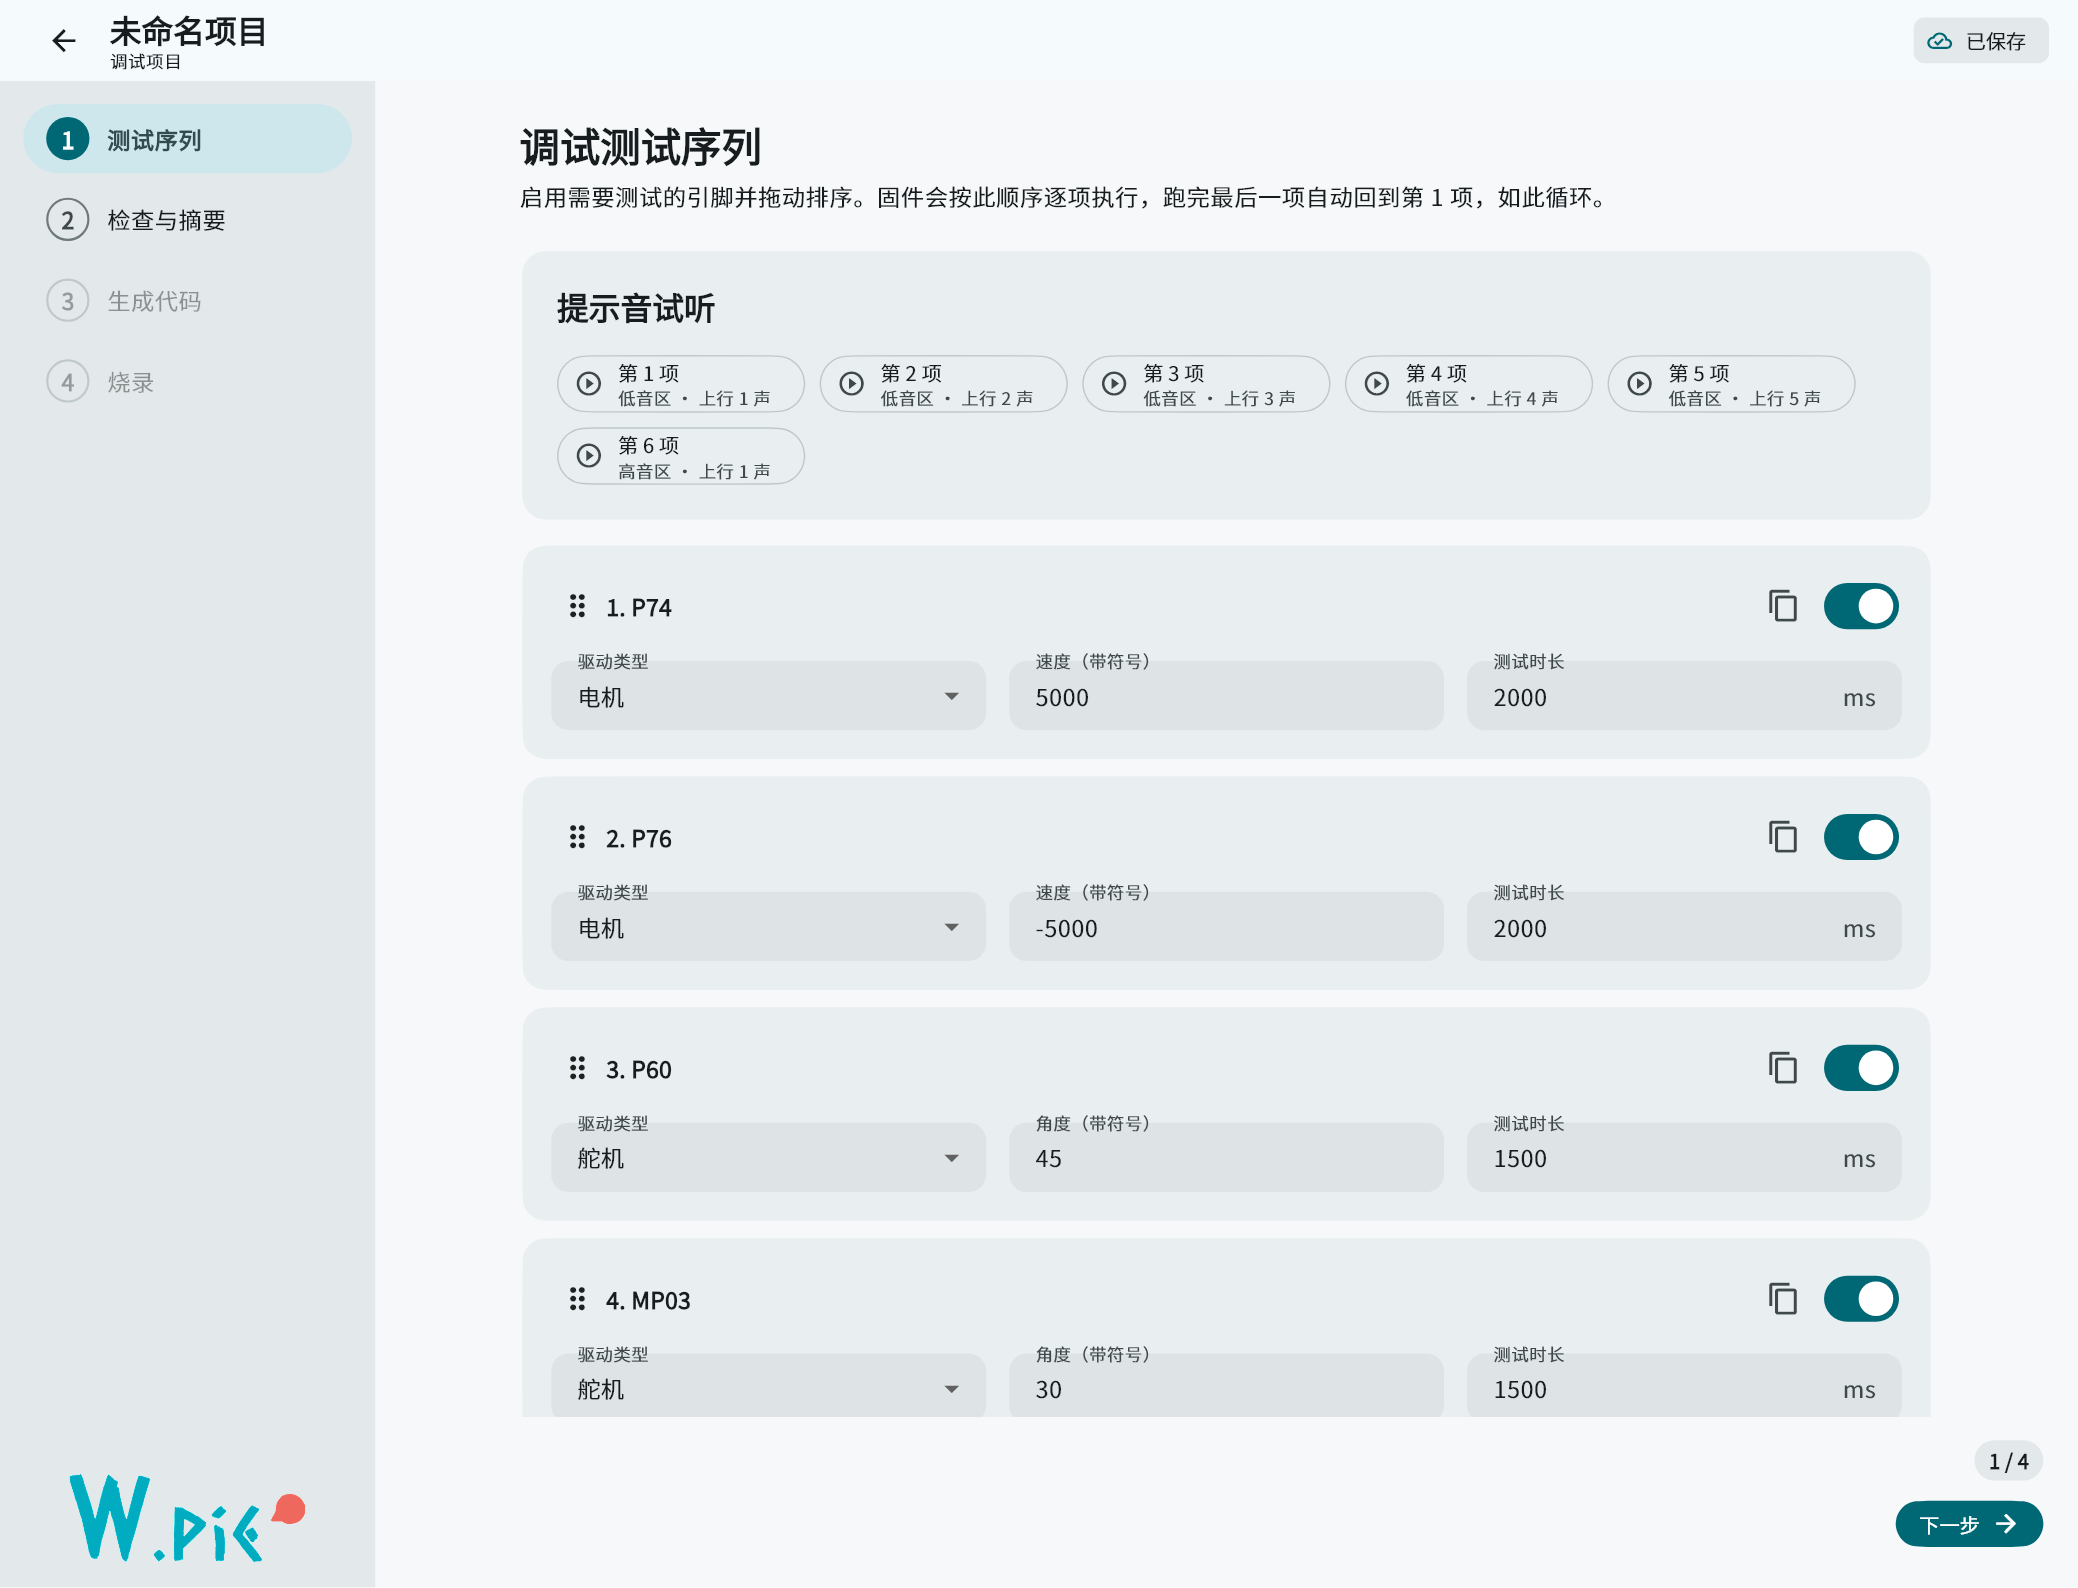
\includegraphics[width=0.95\linewidth]{image/ch06/6-1-debug-tests.png}
  \caption{调试项目的“测试序列”页：上方为提示音试听，下方为按执行顺序排列的测试项}
  \label{fig:concise-debug-tests}
\end{figure}

每个启用的测试项按驱动类型填写：

\begin{itemize}
  \item \textbf{电机}：速度（带符号）与测试时长。正数按默认方向，负数反向，用于在不改
        接线的情况下纠正转向；
  \item \textbf{舵机}：角度（带符号）与测试时长。角度相对中位，方向由正负号决定；
  \item \textbf{摩擦轮}：仅在摩擦轮端口可选，填写目标转速，不填时长。摩擦轮项自带启动
        与渐变流程，执行时自动完成。
\end{itemize}

左侧的拖动手柄用于调整顺序，固件按列表顺序逐项执行，每项结束输出归零，跑完最后一项
自动回到第 1 项循环。需要分段验证同一路时，点击该项右侧的复制键，在下方插入一条相同
配置，再修改数值或时长即可。

装车检查建议按“从轮子到武器”的顺序排列：四个轮电机、云台舵机、摩擦轮。摩擦轮放在最后，
前面任何一项异常都可以直接断电。

页面上方的“提示音试听”把第 $N$ 项对应到上行音型的第 $N$ 个音。装车后即使看不到屏幕，
也可以凭声音判断当前执行到第几项。

\section{检查与摘要}

点击“下一步”进入“检查与摘要”页（图~\ref{fig:concise-debug-review}）。检查结果分为错误与
警告：错误阻止生成，警告只作提示。示例配置只有一项，结果为 0 错误、0 警告，页面提示
“配置检查通过，可以生成代码”。

\begin{figure}[htbp]
  \centering
  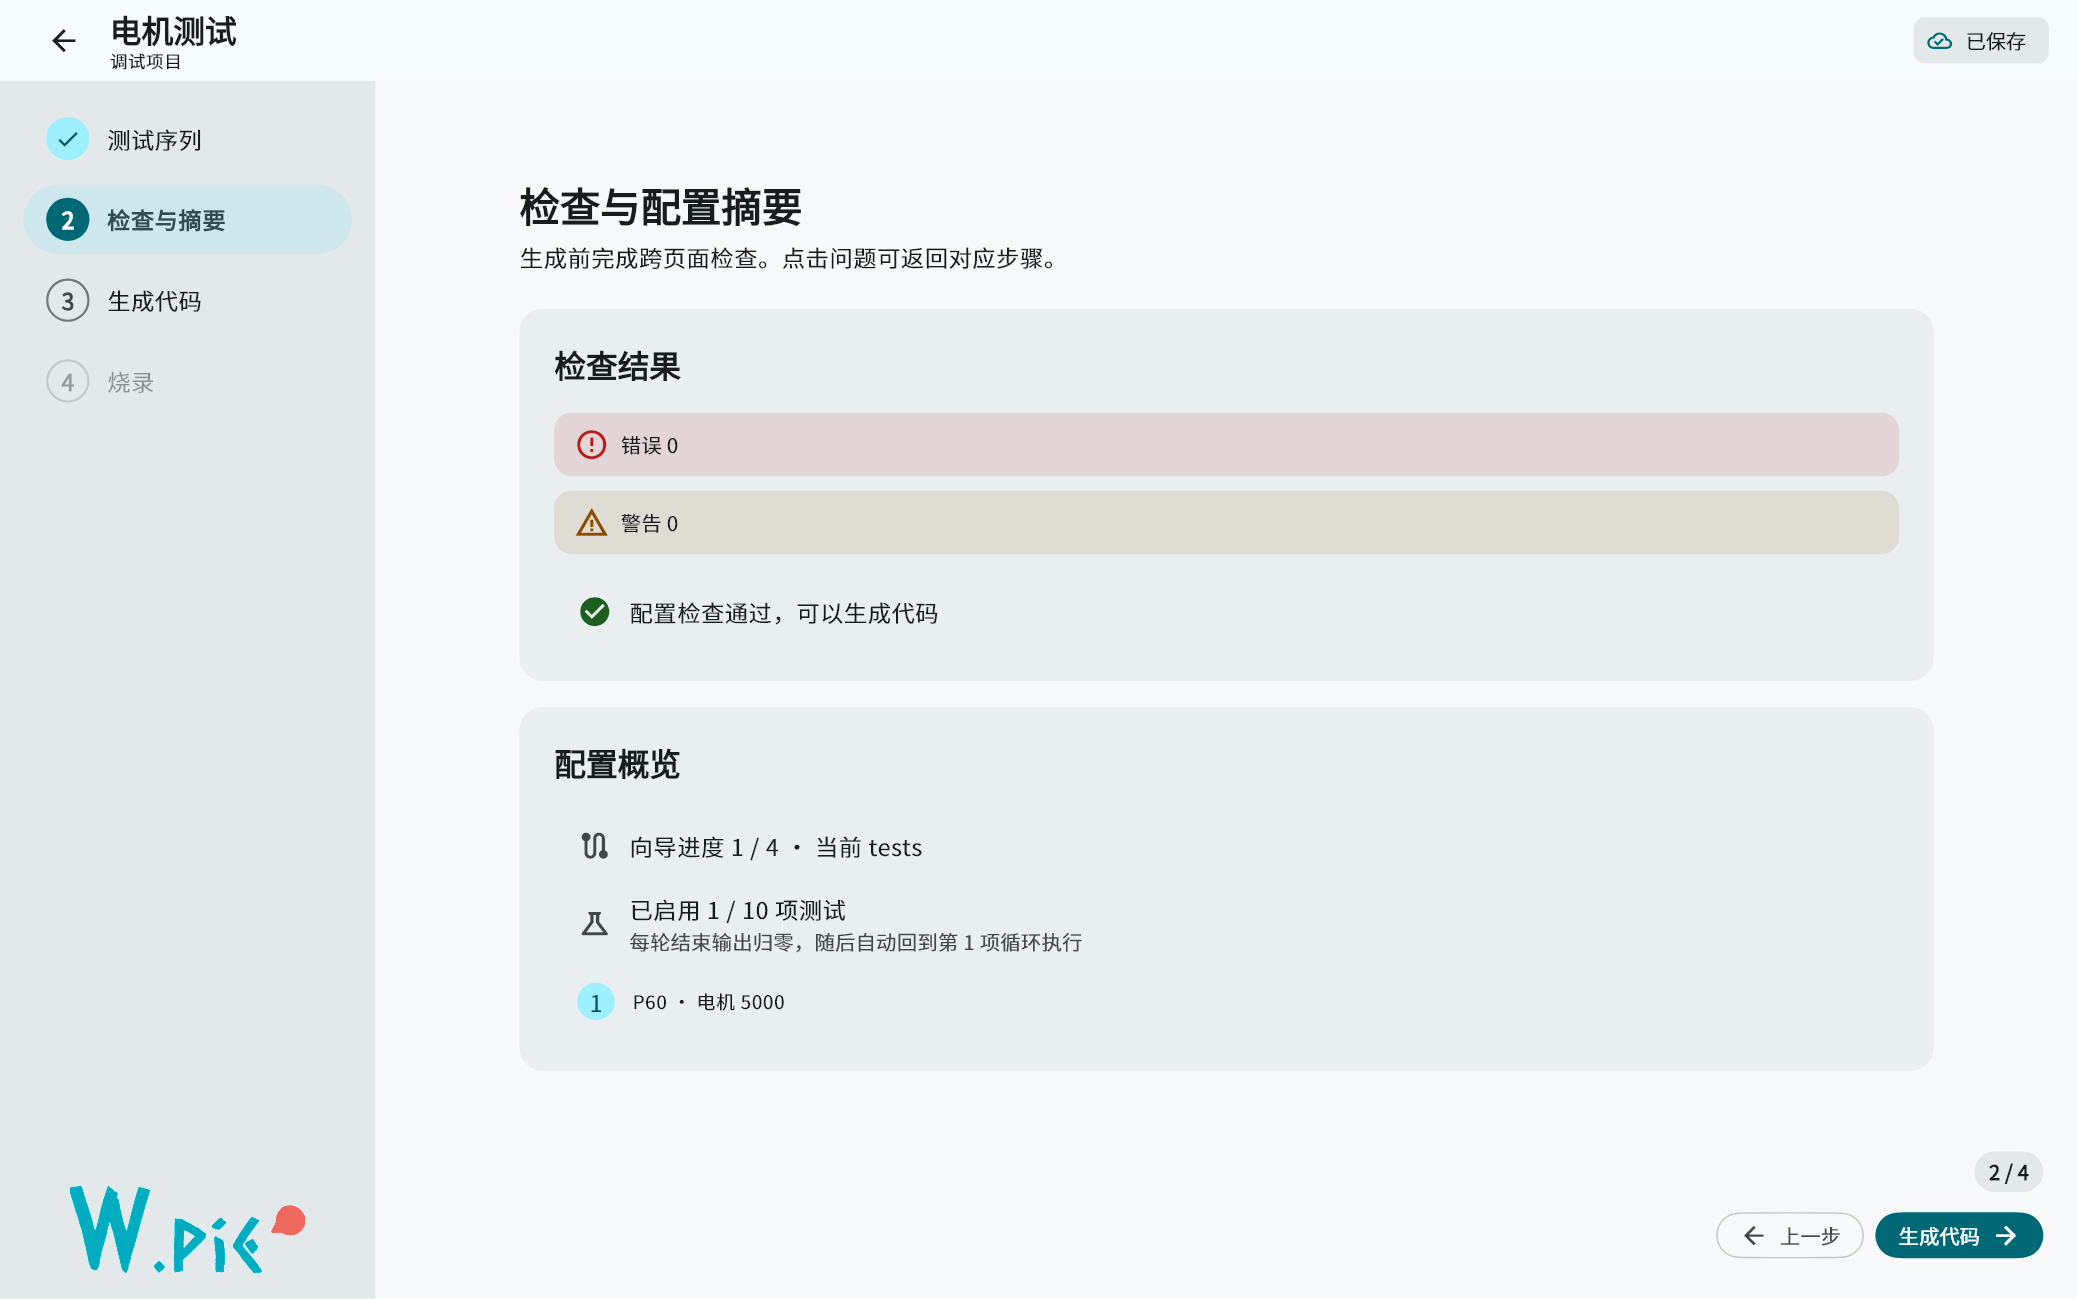
\includegraphics[width=0.95\linewidth]{image/ch02/2-2-review.png}
  \caption{“检查与摘要”页：问题计数与配置概览}
  \label{fig:concise-debug-review}
\end{figure}

“配置概览”汇总已启用的项数与每一项的摘要，供生成前最后核对。若有问题，点击列表中的
条目可直接跳回对应页面；修改后返回检查页，计数随之更新。

\section{编译与烧录}

进入“烧录”页（图~\ref{fig:concise-debug-deploy}）。编译器一栏保持默认的内置编译器即可。
“构建产物”显示编译结果与产物大小；“编译并烧录”完成编译并写入主控板，“仅编译”只验证
配置与编译环境。

\begin{figure}[htbp]
  \centering
  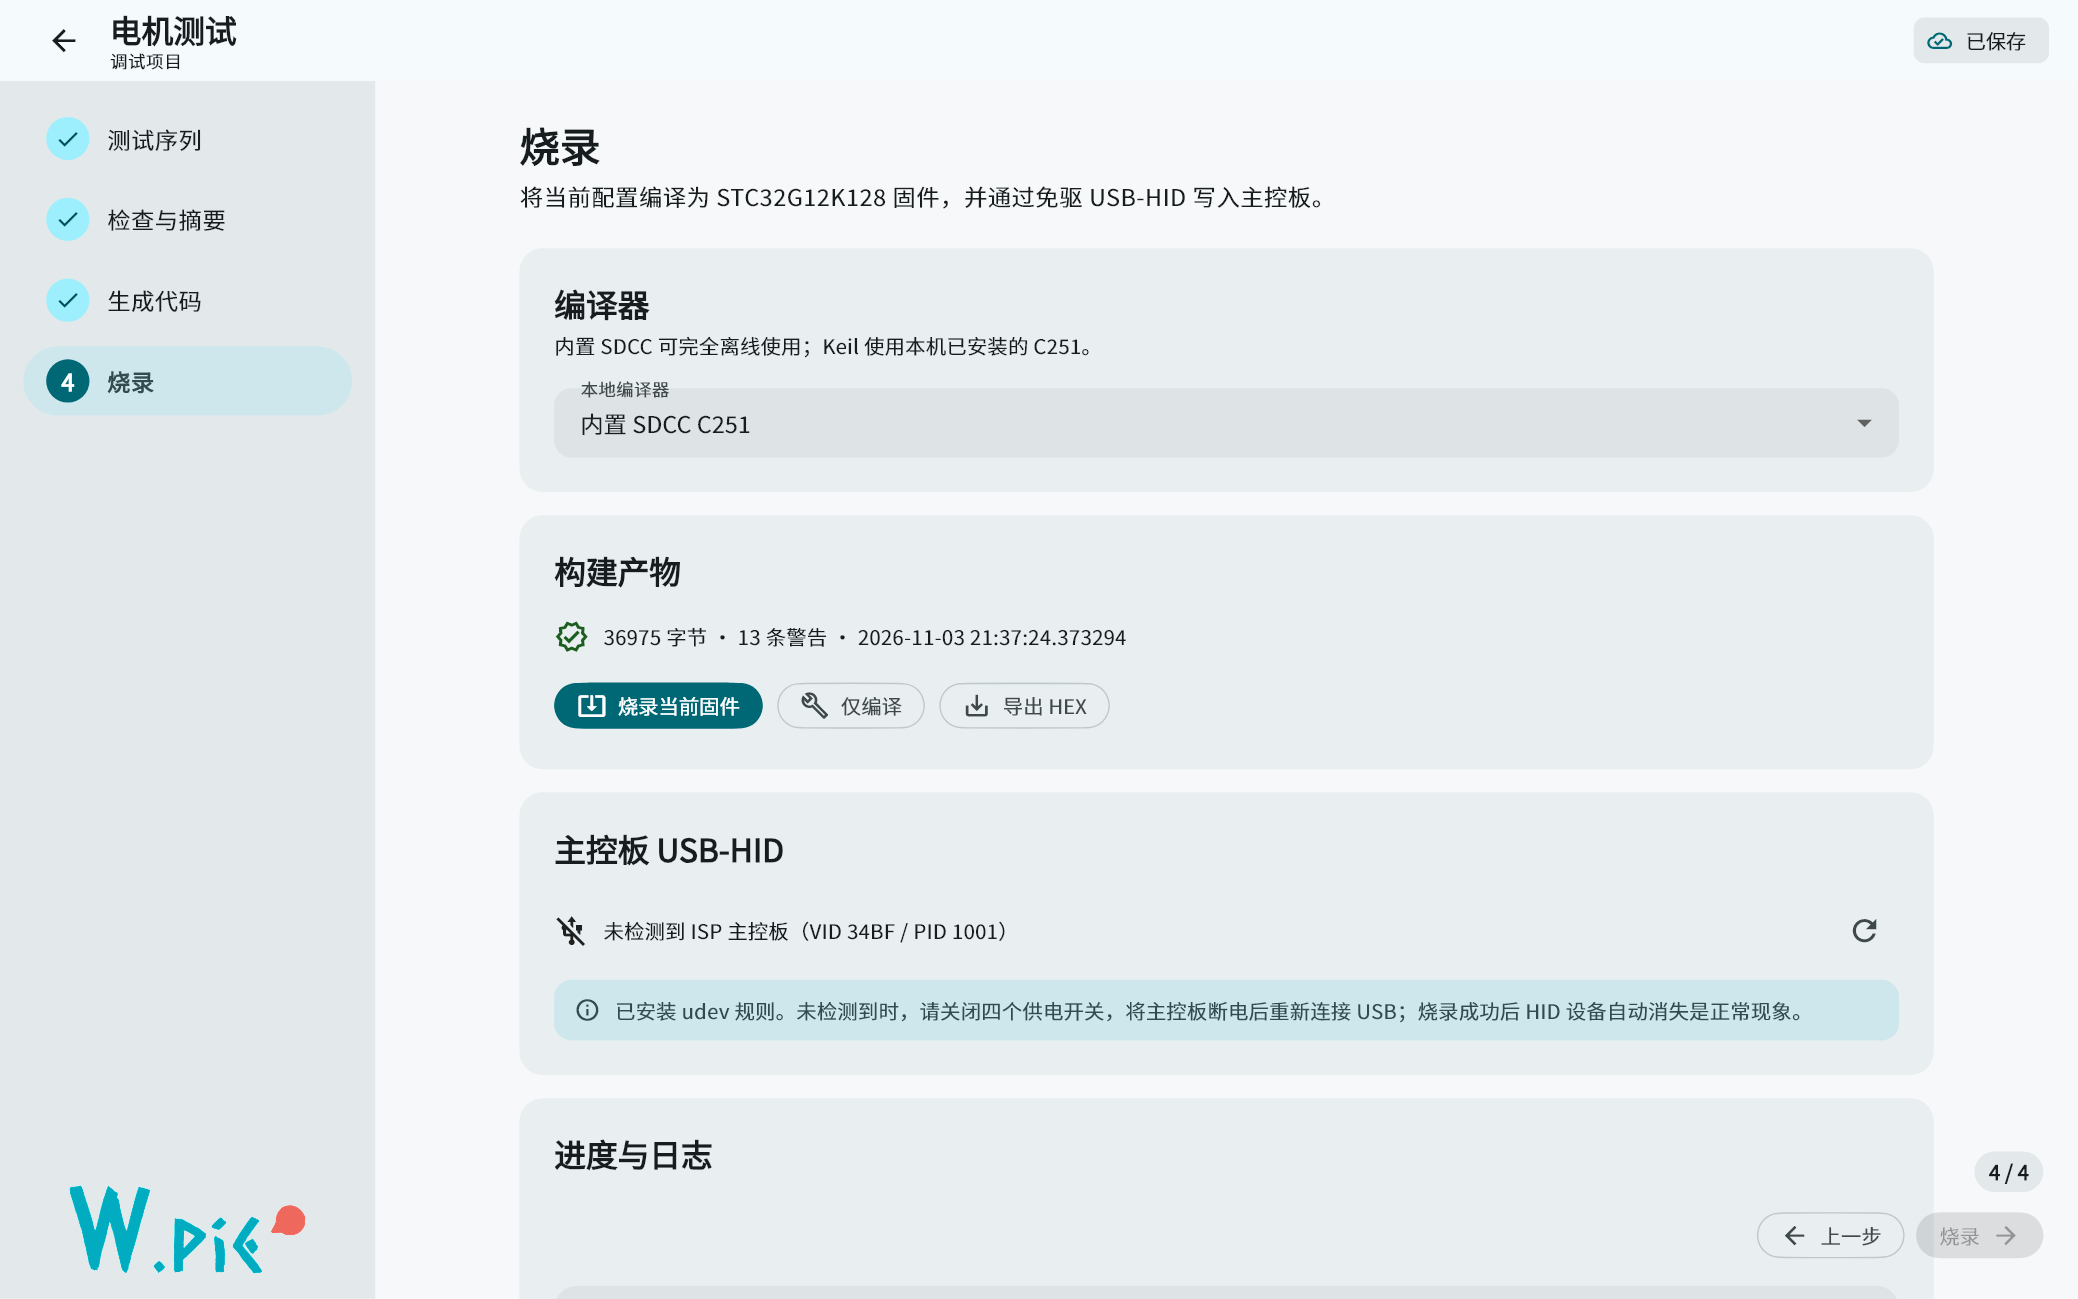
\includegraphics[width=0.95\linewidth]{image/ch02/2-4-deploy.png}
  \caption{“烧录”页：编译器、构建产物、主控板检测与进度日志}
  \label{fig:concise-debug-deploy}
\end{figure}

烧录前完成以下准备：

\begin{enumerate}
  \item 关闭主控板 SERVO、POWER 与机械拓展板 POWER、BOOSTER 四个供电开关；
  \item 将主控板断电，再通过 USB 连接电脑并重新上电，使其进入烧录状态；
  \item 页面检测到主控板后，“编译并烧录”按钮可用。
\end{enumerate}

烧录过程中的进度与日志显示在页面下方。烧录成功后设备会自动复位，检测到的烧录设备消失，
属于正常现象。再次烧录前需要重新断电、上电。

\begin{note}
只能烧录主控板。机械拓展板不运行用户固件，向拓展板烧录会破坏其出厂程序。
\end{note}

\section{上电观察}

烧录完成后接通电源，主控板播放启动提示音，随后按测试序列逐项执行。观察要点：

\begin{itemize}
  \item 每一项是否按设定的方向与时长动作，结束后是否停止；
  \item 提示音的个数是否与当前项序号一致；
  \item 跑完最后一项后是否自动回到第 1 项循环。
\end{itemize}

若某一项方向相反，回到测试序列把该项数值改为相反的符号，重新编译烧录即可，不需要
更改接线。若某一项完全不动作，依次检查供电开关、接线与烧录是否成功。调试项目不使用
遥控器，因此不涉及通道号与死区。

\chapter{步兵项目}
\label{ch:concise-infantry}

\begin{introduction}
  \item 配置遥控器通道、死区与四轮底盘；
  \item 配置云台两个轴、拨弹电机与摩擦轮；
  \item 分配按键并完成方向校准；
  \item 完成检查、编译、烧录与首次上车核对。
\end{introduction}

步兵项目是校内赛最常用的构型：四轮底盘负责移动，云台负责瞄准，拨弹电机把弹丸送入
摩擦轮，摩擦轮把弹丸射出。向导共六步：遥控器与底盘、云台与拨弹、控制与摩擦轮、
检查与摘要、生成代码、烧录。

\section{遥控器与底盘}

\subsection{手柄与通道号}

智能交互手柄通过无线模块与主控板通信，面板包括左右摇杆、A--E 字母按键、四个方向键、
重置键与通道号查看键（图~\ref{fig:concise-handle}）。两只摇杆本身也可以按下，分别记作
LC 与 RC；摇杆的水平与竖直方向提供 LX、LY、RX、RY 四个轴输入。

\begin{figure}[htbp]
  \centering
  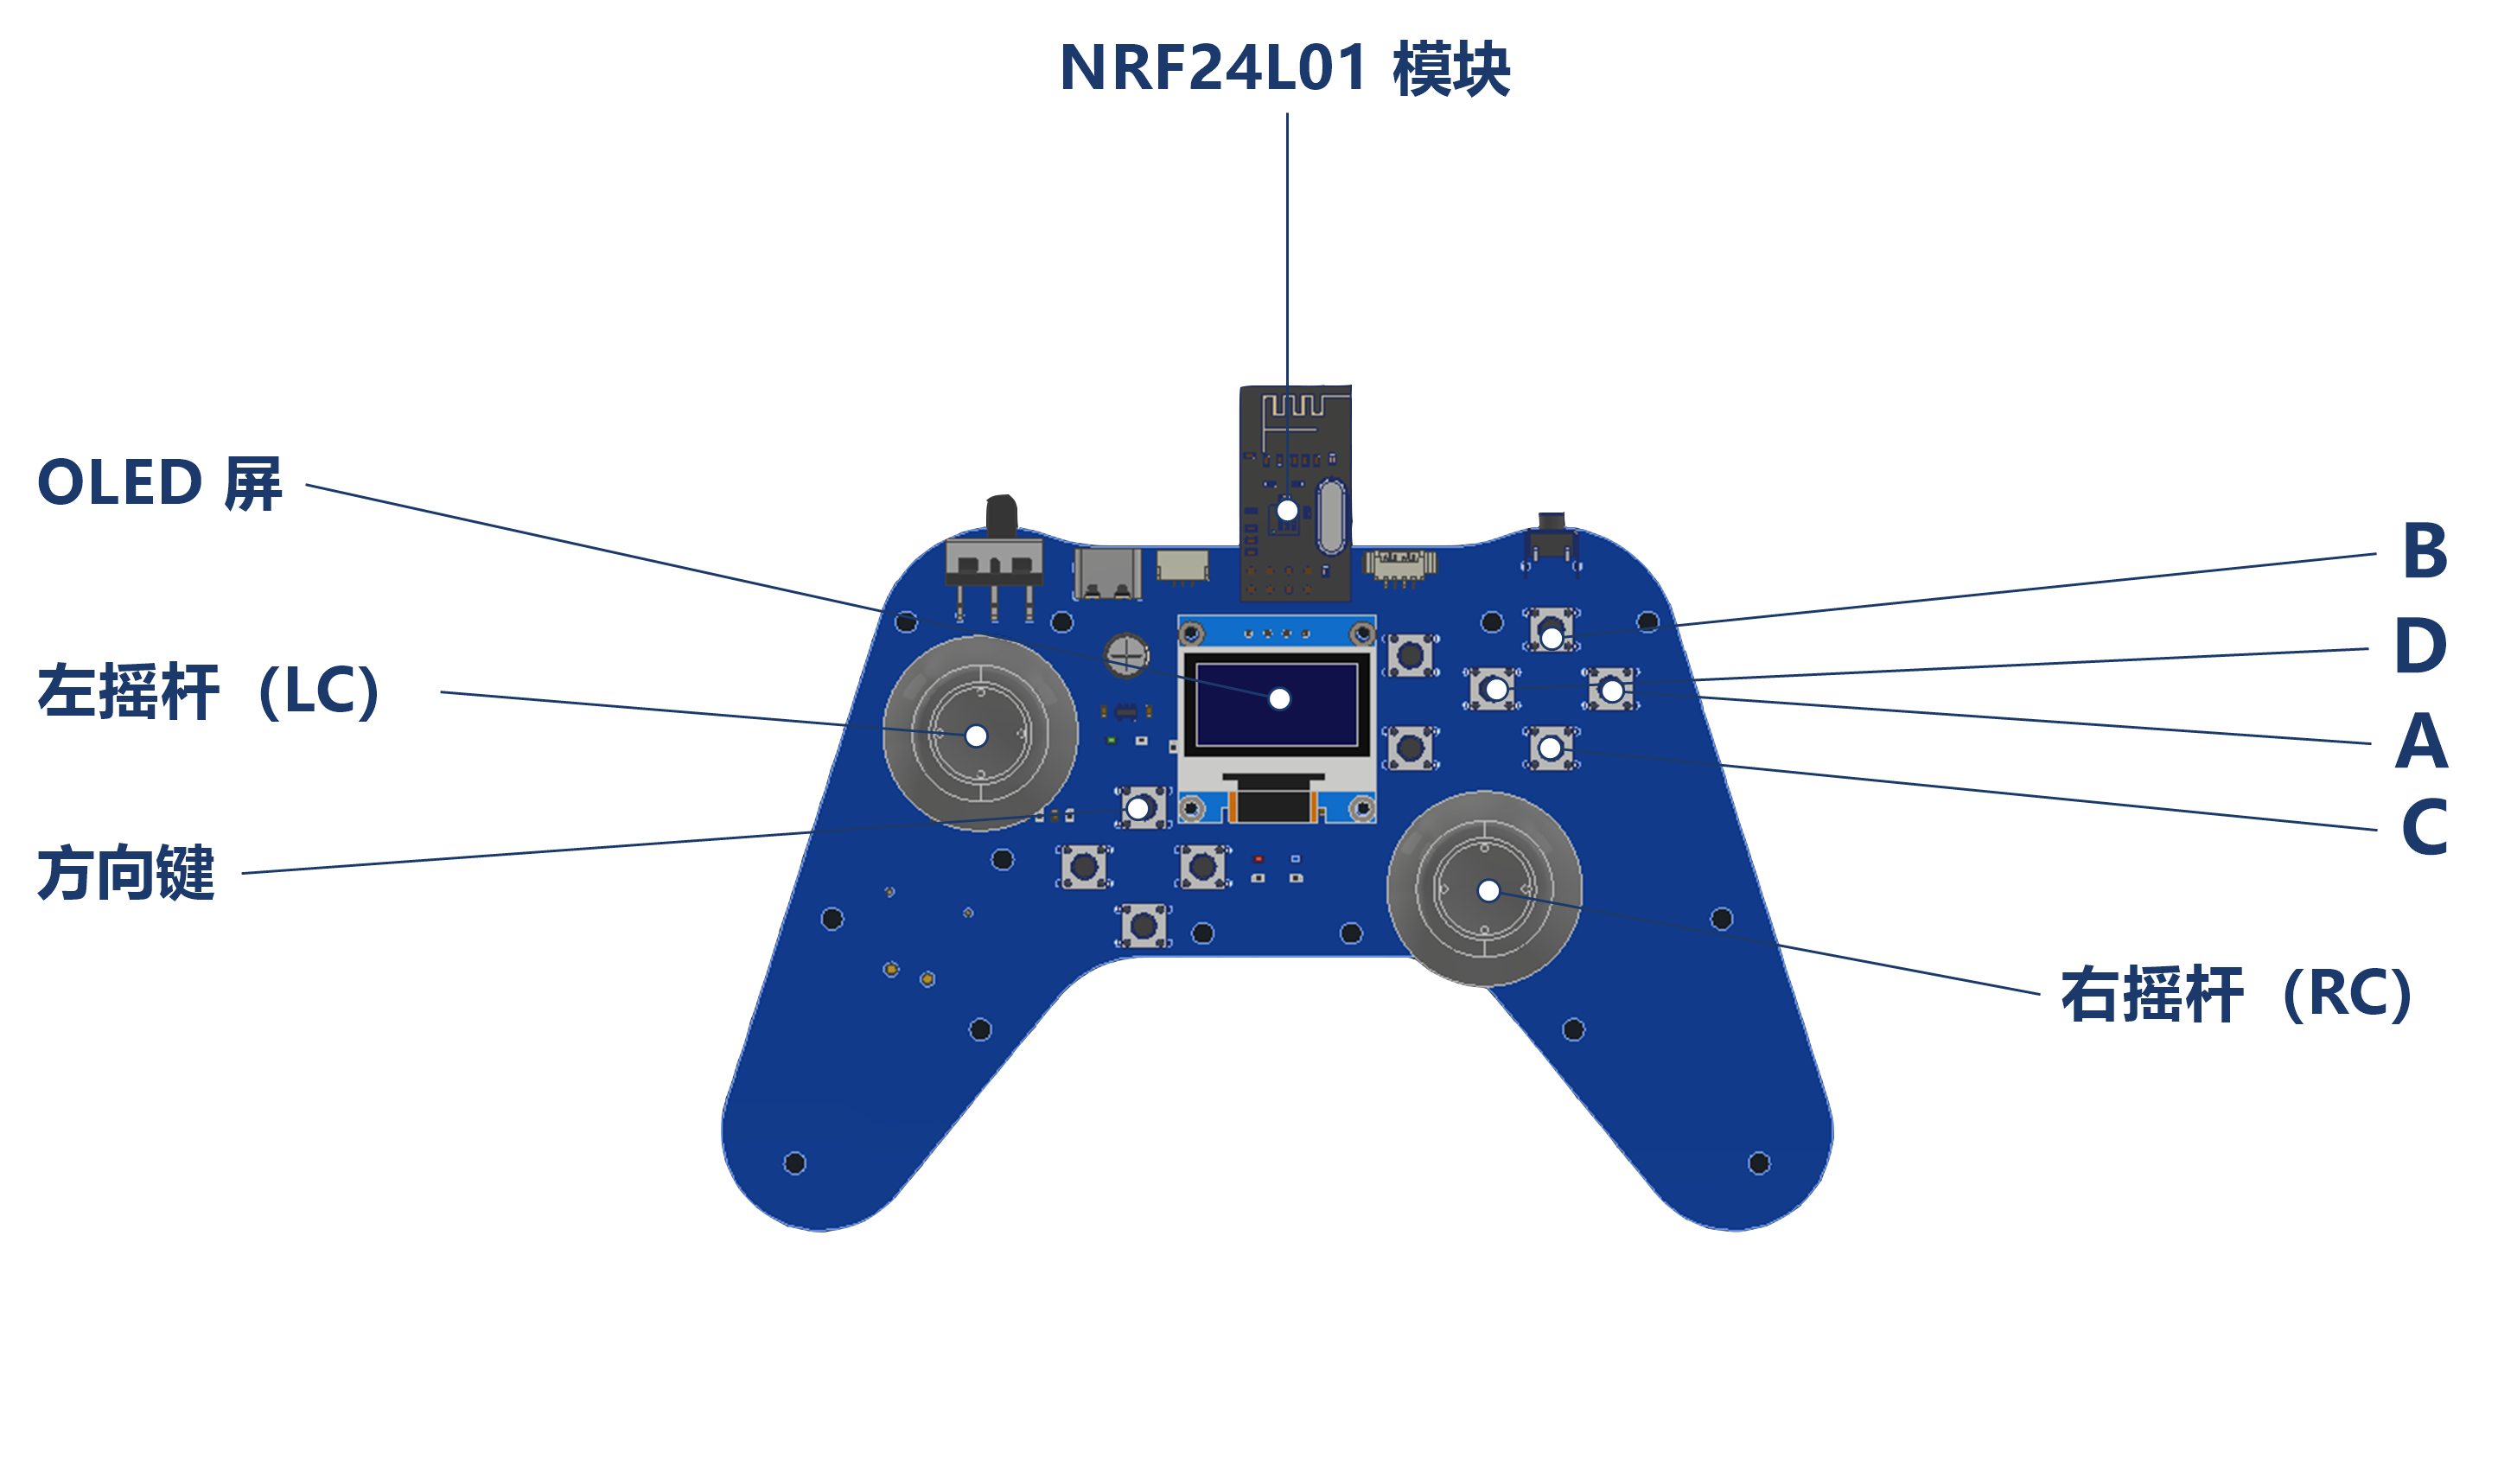
\includegraphics[width=0.98\linewidth]{image/ch03/handle-layout.png}
  \caption{智能交互手柄面板：双摇杆、字母按键、方向键与 OLED 屏}
  \label{fig:concise-handle}
\end{figure}

手柄与主控板必须使用同一个通道号。手柄开机后长按通道号查看键，屏幕显示当前通道号；
把该数字填入“遥控器与底盘”页的“通道号”一栏即可。通道不一致时主控板收不到任何数据，
这是“车完全不动”的首要排查项。

“摇杆死区”用于忽略摇杆回中后的微小偏移。死区太小，底盘可能在无操作时缓慢漂移；死区
太大，小幅推杆没有反应，操控显得迟滞。取值范围为 0--2047，建议不超过 500，100 是常用
的起始值。

\subsection{四轮与方向}

“四轮底盘”区按左前、左后、右前、右后分别选择 IO 与方向
（图~\ref{fig:concise-remote}）。IO 下拉框只列出当前可用的电机端口；同侧前后轮可以共用
一个 IO，但共用时两轮方向必须相同。

\begin{figure}[htbp]
  \centering
  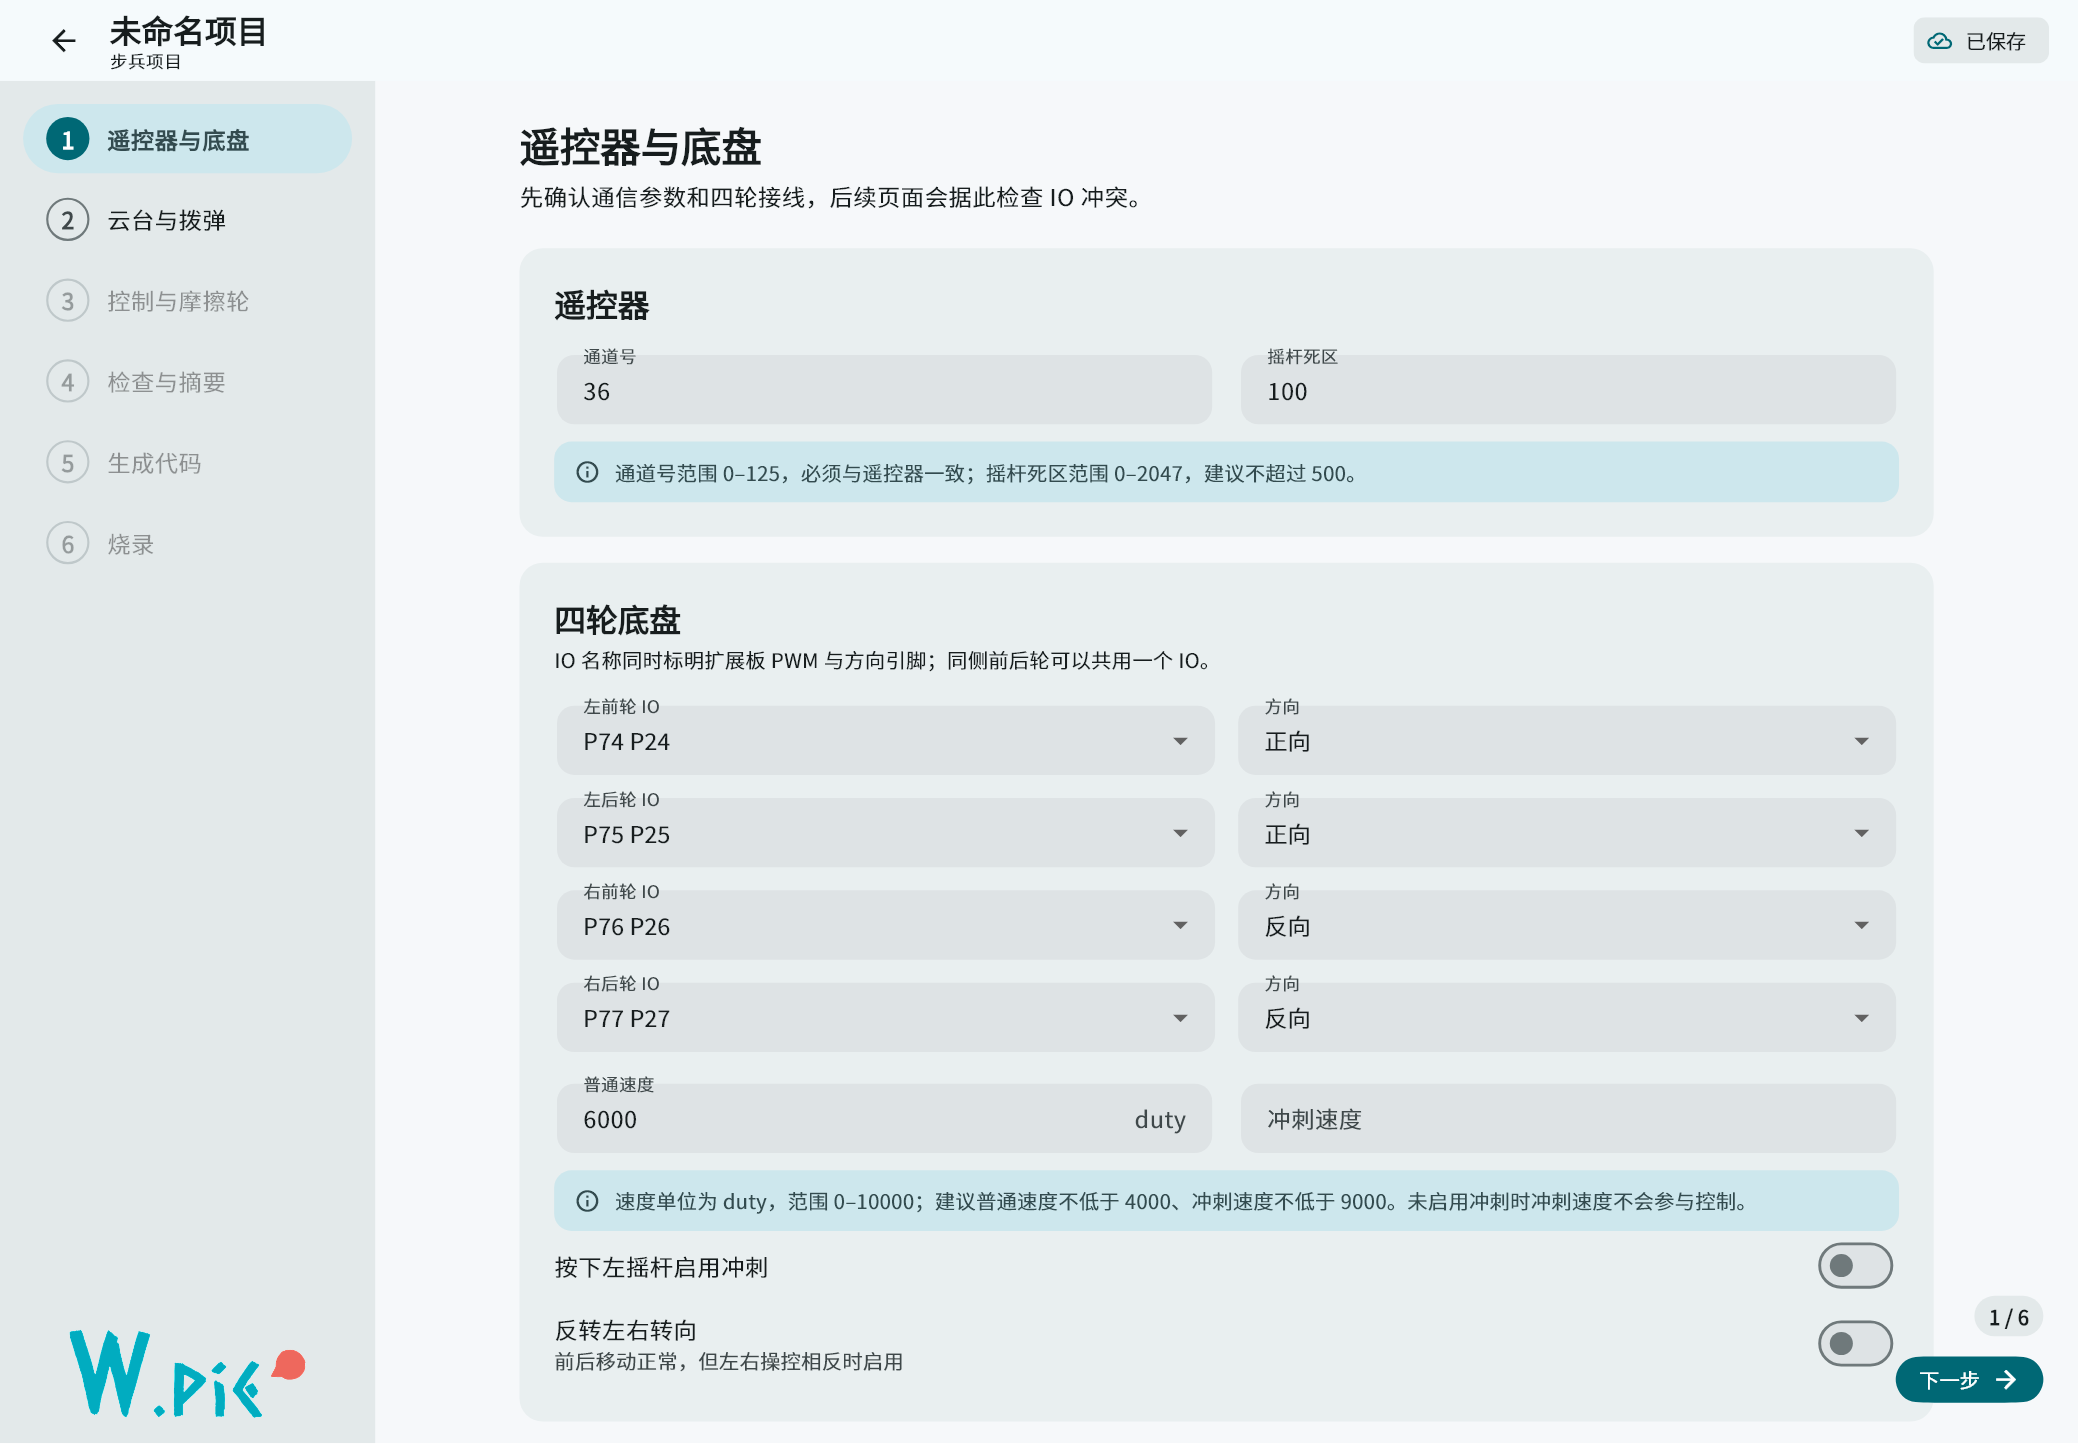
\includegraphics[width=0.98\linewidth]
    {image/ch03/3-1-remote-top.png}
  \caption{“遥控器与底盘”页：通道、死区、四轮 IO 与方向、普通与冲刺速度}
  \label{fig:concise-remote}
\end{figure}

“方向”表示该路电机的安装与接线是否符合默认约定。最常见的情形是右侧电机镜像安装，
因此右侧两轮通常设为“反向”，左侧两轮设为“正向”。装配后若某个轮子的转向与预期相反，
修改该轮的方向即可，不需要更改接线。

\subsection{速度与操控}

“普通速度”是左摇杆推满时的底盘速度，建议不低于 4000；“冲刺速度”是按住冲刺键时的
速度，建议不低于 9000，且不得小于普通速度。两者取值范围均为 0--10000。

打开“按下左摇杆启用冲刺”后，按下左摇杆即切换到冲刺速度，松开恢复普通速度。若前后
移动正常、左右转向相反，打开“反转左右转向”即可，不必改动电机接线。

\subsection{方向校准}

首次上车按下述顺序核对，全程架空并临时降低普通速度：

\begin{enumerate}
  \item 轻推左摇杆向上，四个轮子应同时向前滚动；某个轮子相反时，修改该轮的方向；
  \item 轻推左摇杆向左，车体应向左转；方向相反时，打开“反转左右转向”；
  \item 按下左摇杆并推满，速度应明显提升；
  \item 确认无误后落地，低速试走直线，再逐步提高速度。
\end{enumerate}

\section{云台与拨弹}

\subsection{云台两个轴}

“云台与拨弹”页把云台分为 Yaw（偏航，水平旋转）与 Pitch（俯仰）两个轴
（图~\ref{fig:concise-mechanism}）。每个轴默认有一个执行器，点击“添加执行器”可以扩展为
多个执行器同步动作。每个执行器填写四项：

\begin{itemize}
  \item \textbf{驱动类型}：舵机或电机；IO 下拉框只给出该类型可用的端口；
  \item \textbf{IO}：执行器所在端口；
  \item \textbf{方向}：纠正安装方向，与底盘单轮方向含义相同；
  \item \textbf{归中偏移}：舵机机械正前方相对中位的角度偏差。舵盘装配难以恰好居中，
        把偏差填在这里，归中位置才会落在机械正前方。
\end{itemize}

“逆时针限幅”与“顺时针限幅”是相对归中位置的两侧可用行程，选填；留空表示该侧走满
可用行程。行程仍受机械限位约束，首次动作应低速、小幅度验证。

云台由右摇杆控制：水平方向驱动 Yaw，垂直方向驱动 Pitch。舵机执行器按转速方式响应，
推杆越深转动越快，松手即停；电机执行器按摇杆幅度输出。打开“按下右摇杆让云台归中”后，
按下 RC 可使两轴回到各自的归中位置。

\begin{figure}[htbp]
  \centering
  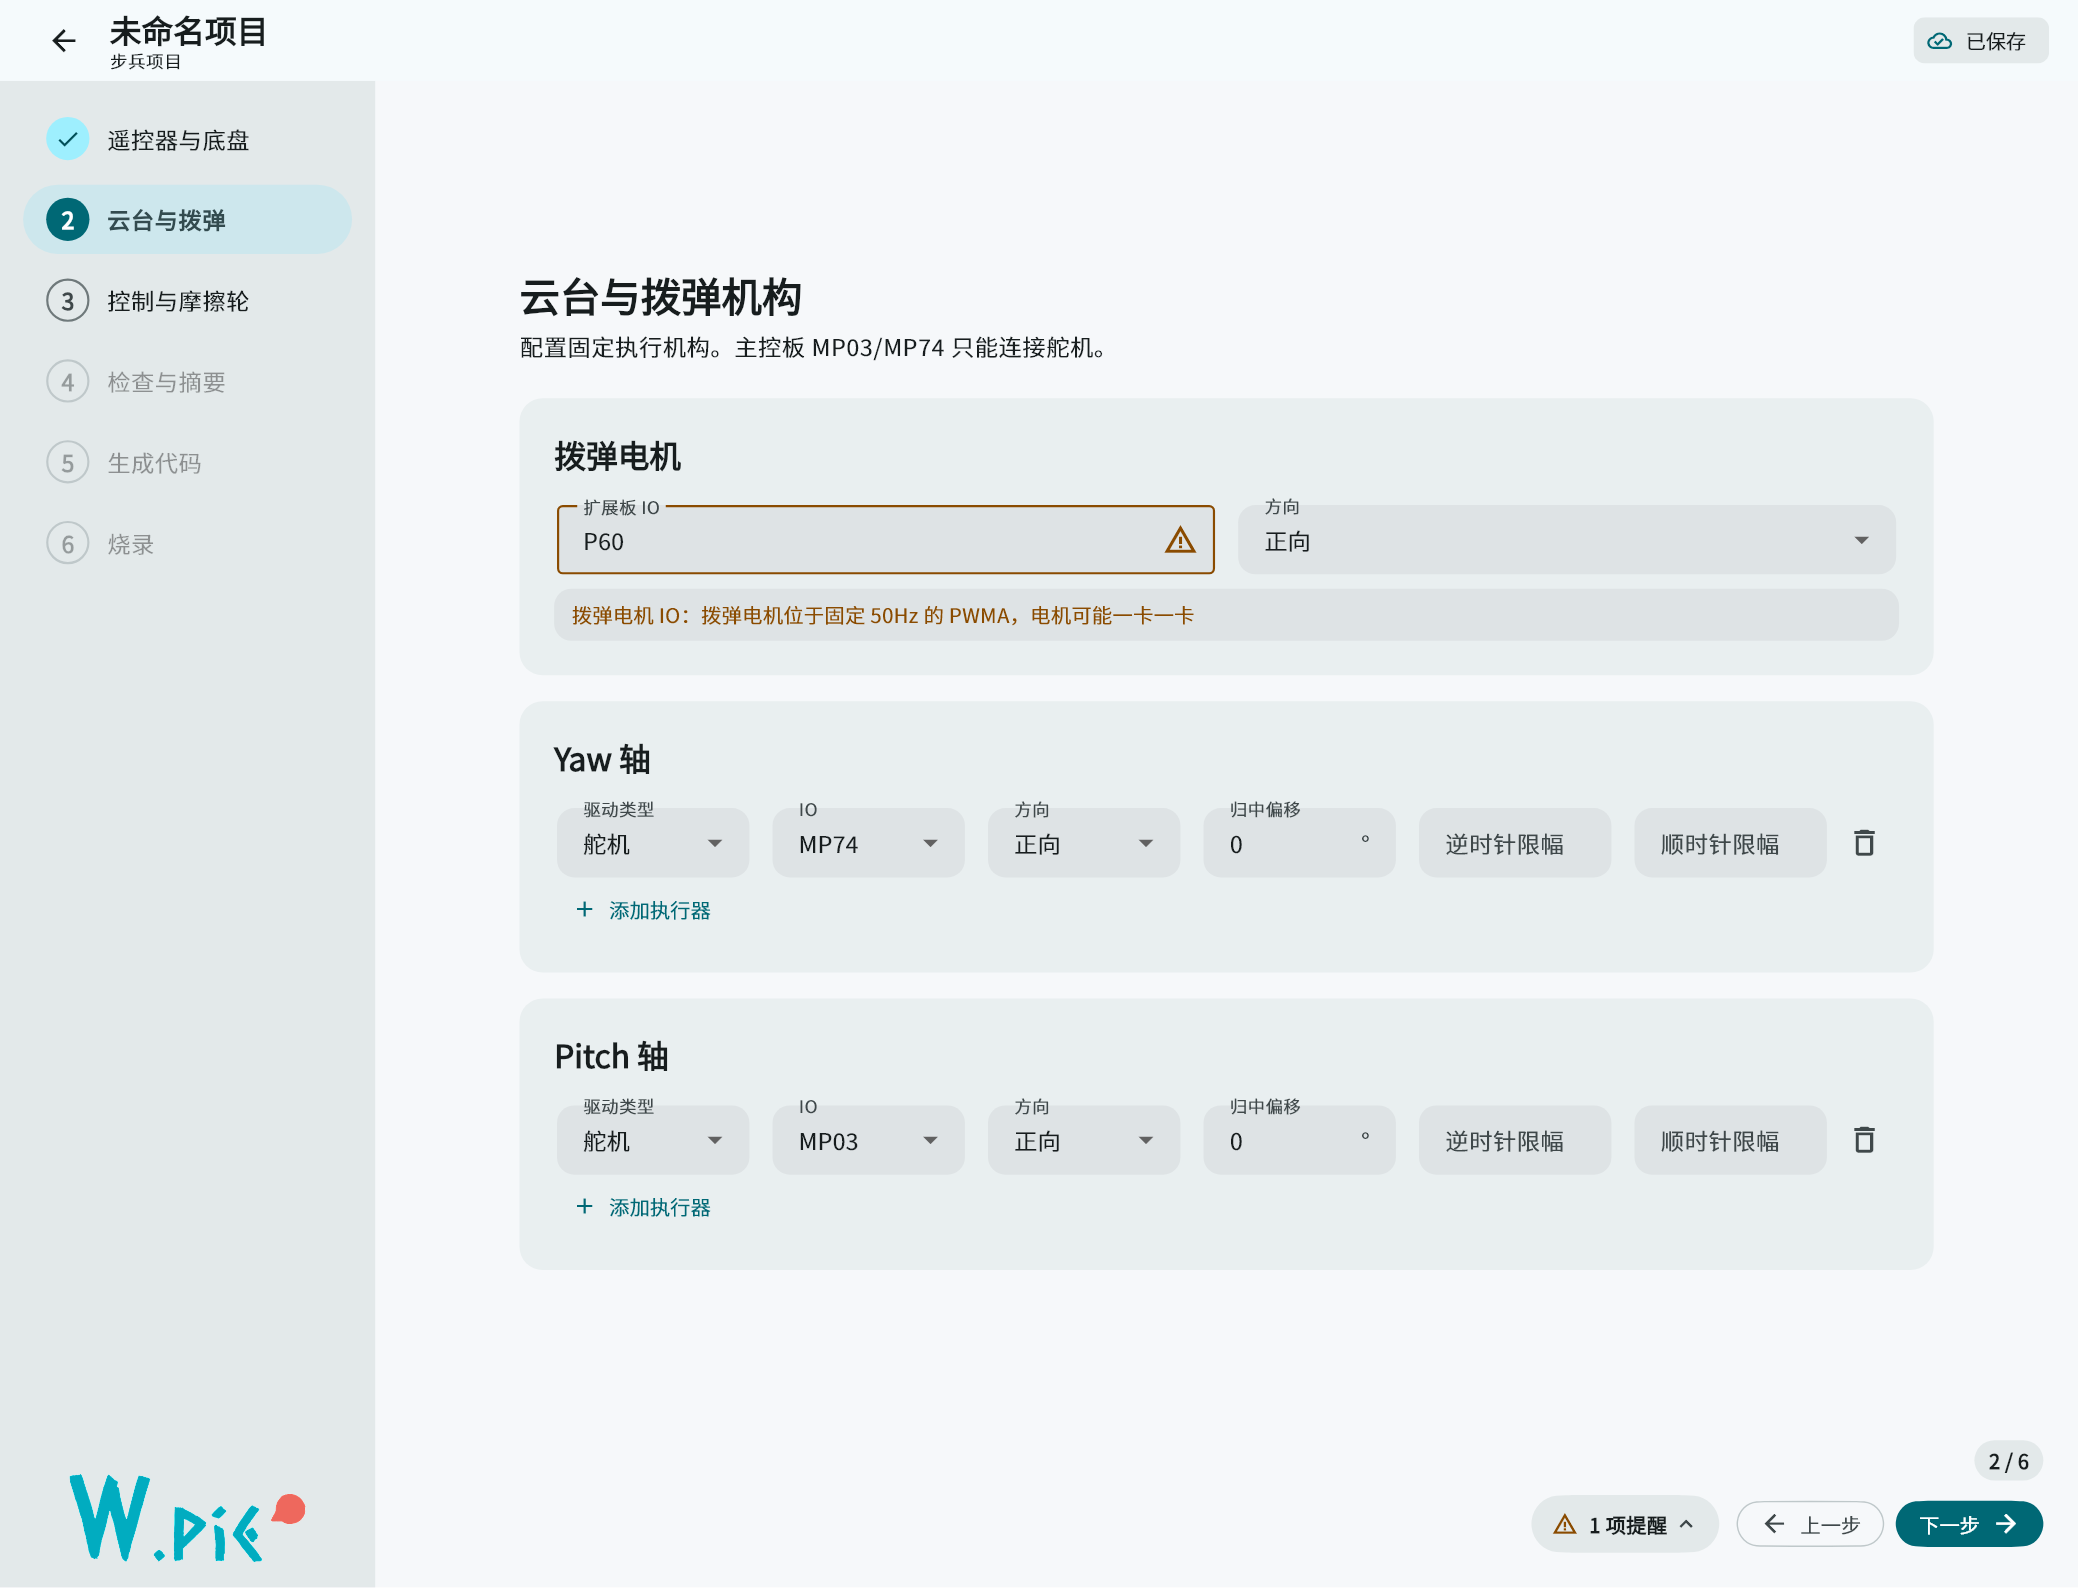
\includegraphics[width=0.98\linewidth]{image/ch04/4-1-mechanism.png}
  \caption{“云台与拨弹”页：拨弹电机、Yaw 轴与 Pitch 轴的执行器参数}
  \label{fig:concise-mechanism}
\end{figure}

\subsection{拨弹电机}

拨弹电机负责把弹丸从弹仓送入摩擦轮。填写 IO 与方向，并选择拨弹模式：

\begin{itemize}
  \item \textbf{阻塞开环单发}：每按一次扳机键，拨弹电机转动一个“单发时长”，送出一颗
        弹丸。单发期间底盘与云台暂停响应，因此单发时长不宜过大，250\,ms 是常用的起始值；
  \item \textbf{目视闭环连续拨弹}：按住扳机键持续拨弹，松开即停，由操作手目视控制节奏。
\end{itemize}

“反向拨弹键”用于卡弹时退弹：按住时按相反方向持续转动，松开立即停止。该键可以留空。

拨弹电机所在的引脚组频率较低，页面可能提示“电机可能一卡一卡”。这属于硬件分组决定的
正常提醒，不是配置错误；适当提高拨弹速度或缩短单发时长可以减轻该现象。

\section{控制与摩擦轮}

\subsection{按键分配}

“控制与摩擦轮”页为拨弹与摩擦轮分配按键（图~\ref{fig:concise-controls}）。同一个数字
按键不能分配给两个动作；启用冲刺后 LC 归底盘使用，启用云台归中后 RC 归云台使用；
方向键按用途占用。冲突会在检查页以错误列出，也可点击条目跳回本页修改。

\begin{figure}[htbp]
  \centering
  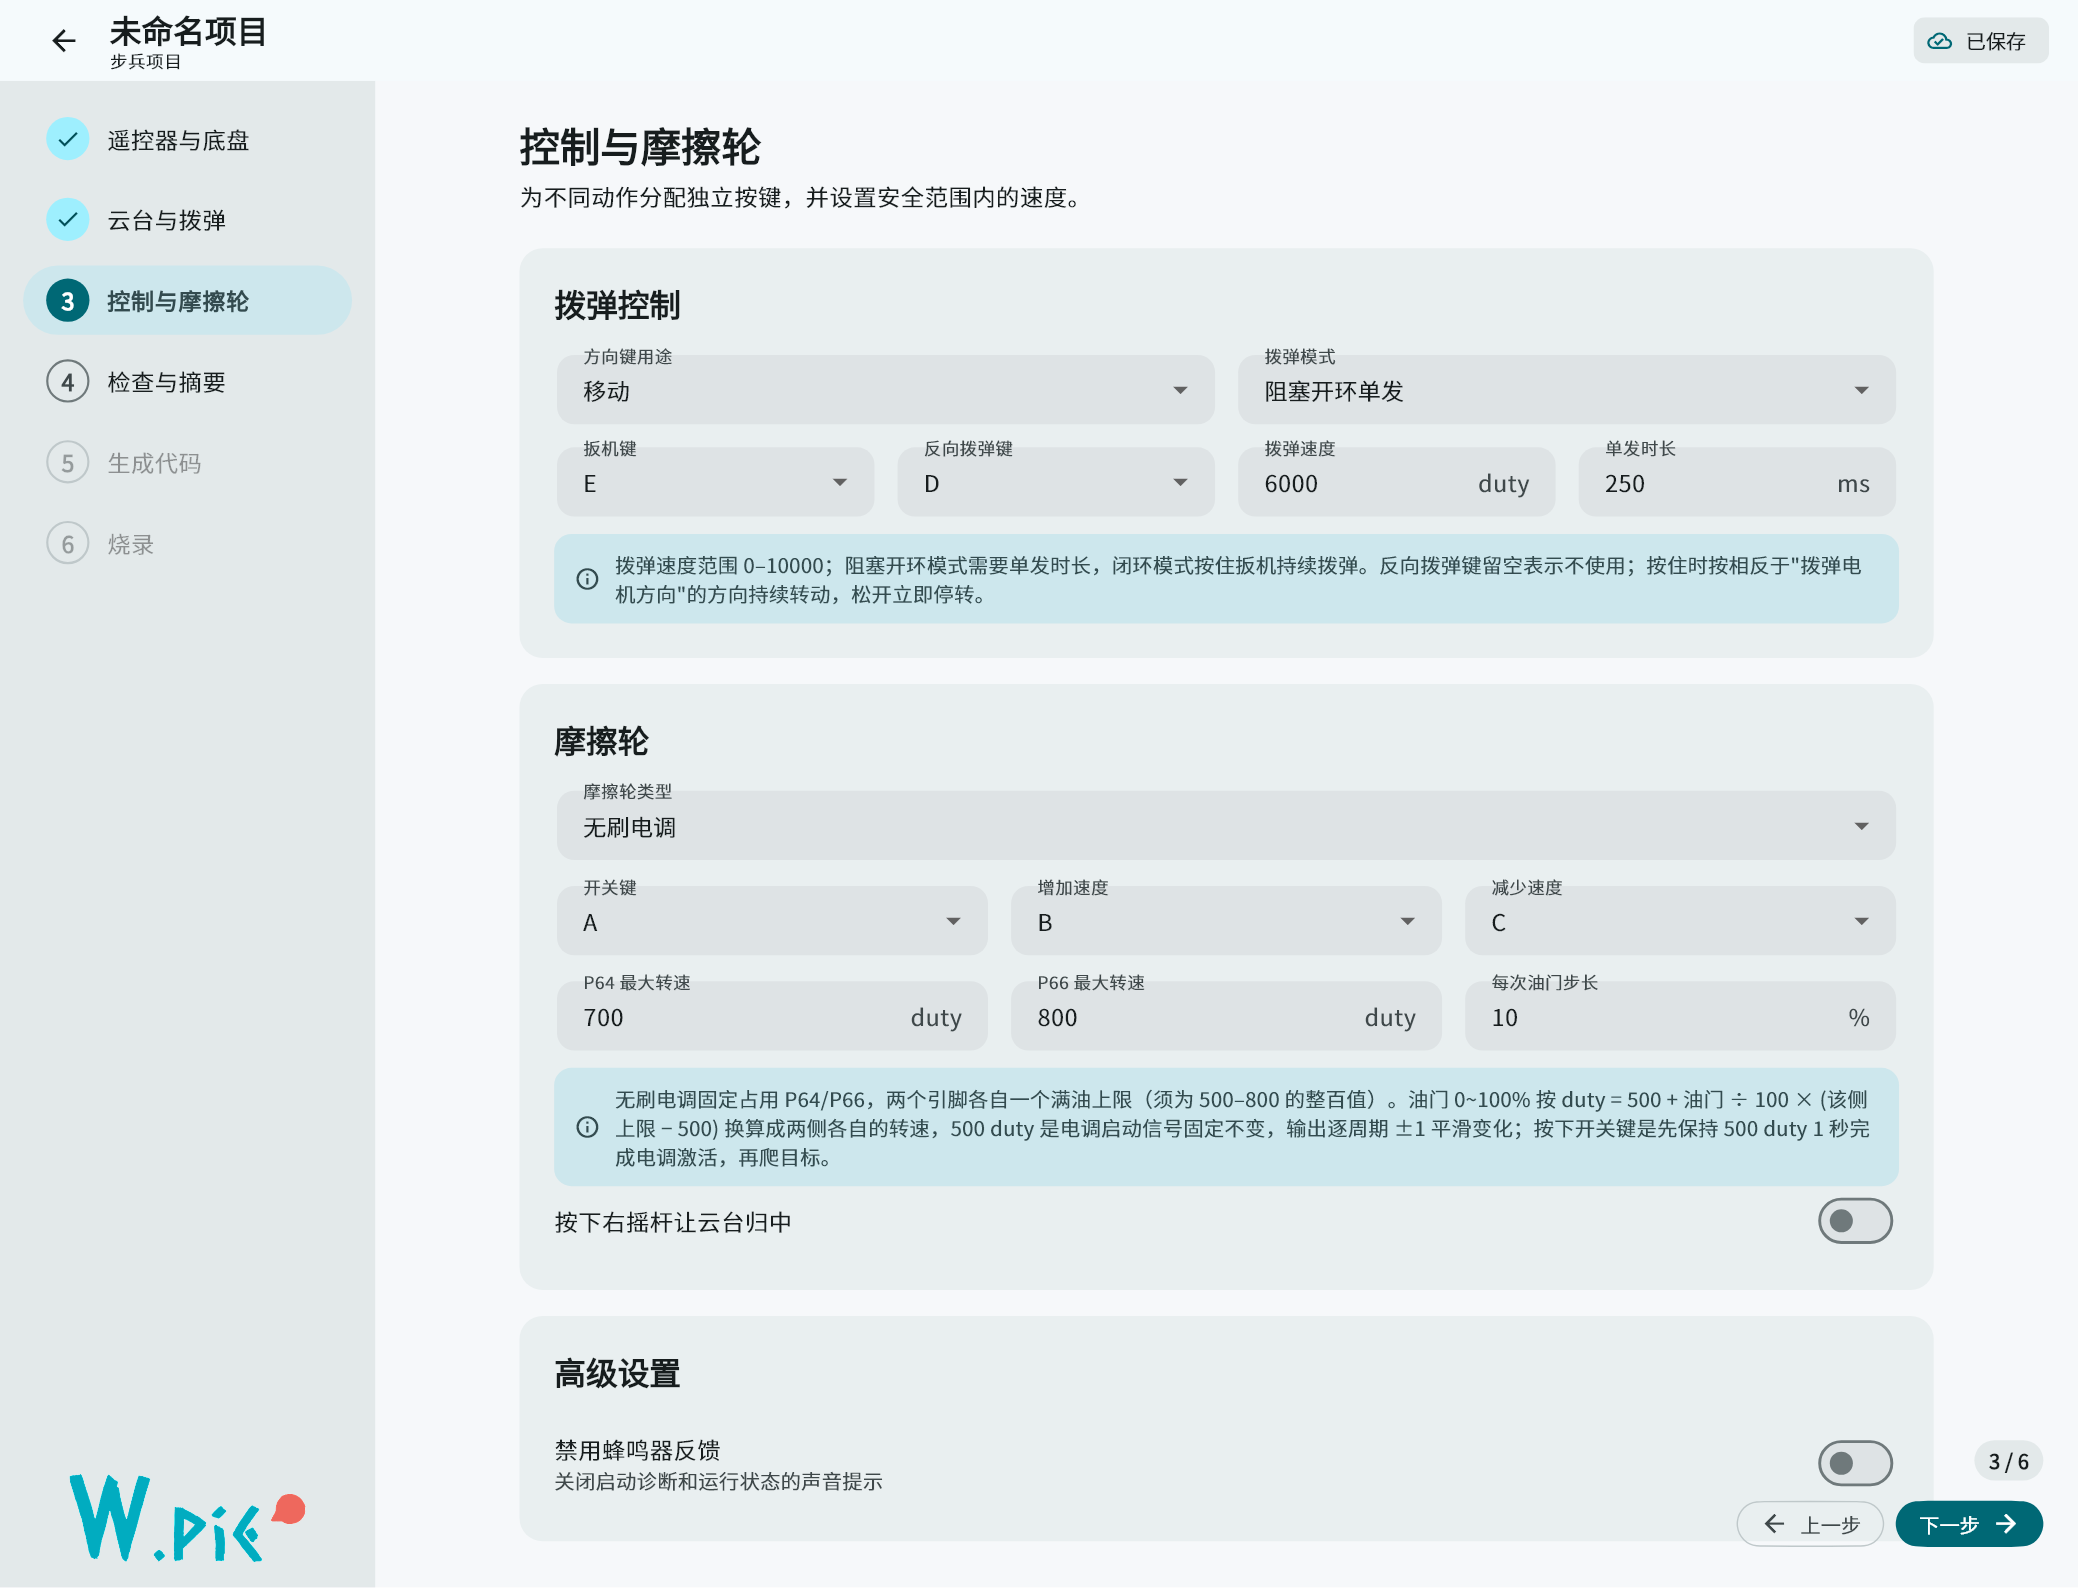
\includegraphics[width=0.98\linewidth]{image/ch04/4-2-controls.png}
  \caption{“控制与摩擦轮”页：拨弹按键与参数、摩擦轮按键与两侧最大转速}
  \label{fig:concise-controls}
\end{figure}

\subsection{摩擦轮}

摩擦轮使用无刷电机与电调，软件把安全规程固化在固件中，界面只暴露油门与最大转速。
摩擦轮类型选择“无刷电调”后固定占用 P64、P66 两个端口；选择“不使用”时释放。

摩擦轮需要三个按键：\textbf{开关键}在停止与当前油门之间切换，\textbf{增加速度键}与
\textbf{减少速度键}按“每次油门步长”调整油门。油门范围为 0--100\%，步长常用 10\%。
两侧分别设置\textbf{最大转速}，取值为 500--800 的整百值，用于补偿两侧机械差异。

摩擦轮的启动与停止由固件按安全流程执行：启动时先以启动转速保持约一秒完成电调激活，
再平滑爬升到目标；停止时沿同一斜坡降回后停止。激活与渐变期间不需要人工干预，也不应在
高速运转时直接切断电源。

两侧最大转速的标定方法：

\begin{enumerate}
  \item 两侧先都填 800，油门步长设为 10\%；
  \item 架空发射机构，人员离开射界，按开关键启动，确认两侧都能平稳起转；
  \item 逐档增加油门，比较两侧声音与弹丸初速；偏慢的一侧适当调高最大转速，或把偏快
        一侧调低；
  \item 确定常用工作点后记录数值，比赛中只调整油门档位，不再修改最大转速。
\end{enumerate}

“高级设置”中的“禁用蜂鸣器反馈”用于关闭上电与状态变化时的提示音，适合安静的调试环境。
该开关不影响摩擦轮的安全流程。

\section{检查、编译与烧录}

三页配置完成后进入“检查与摘要”。除错误外，步兵项目常见的警告包括：冲刺速度低于建议值、
拨弹电机位于低频引脚组、摩擦轮最大转速偏低等。警告不阻止生成，但应逐条确认是否符合
实际方案。

编译与烧录的步骤与第~\ref{ch:concise-debug}~章一致：关闭四个供电开关，主控板断电后
重新连接 USB，检测到设备后点击“编译并烧录”。烧录完成后按附录~\ref{app:concise-check}
的检查单逐项核对，再落地低速试走。

\begin{note}
步兵固件同时驱动底盘、云台、拨弹与摩擦轮。首次上电应架空并清空弹仓；确认底盘方向、
云台行程与摩擦轮启停均正常后，才可安装弹丸并落地运行。
\end{note}

\chapter{工程项目}
\label{ch:concise-engineer}

\begin{introduction}
  \item 了解工程项目的适用场景与向导步骤；
  \item 会设置引脚角色与多套控制模式；
  \item 会用动作行与动作表安排按键动作；
  \item 按架空、低速、逐项的顺序完成实车验证。
\end{introduction}

工程项目用于预制四轮底盘无法覆盖的构型：麦克纳姆轮底盘、全向轮底盘、机械臂，以及
底盘与作业机构组合的机器人。它把控制方式交给使用者安排：先确定每个引脚做什么，再为
每个按键或摇杆安排动作。自由度更高，实车验证也更重要。

\section{适用场景}

表~\ref{tab:concise-engineer-configs} 列出校内赛常见的工程构型与配置要点。运动学关系
不需要手工推导，按动作行逐路安排摇杆与按键即可。

\begin{table}[htbp]
  \centering
  \small
  \begin{tabularx}{\linewidth}{@{}>{\raggedright\arraybackslash}p{0.20\linewidth}
      >{\raggedright\arraybackslash}p{0.30\linewidth}
      >{\raggedright\arraybackslash}X@{}}
    \toprule
    构型 & 特点 & 配置要点 \\
    \midrule
    四轮麦克纳姆轮 & 可前后、左右平移与原地旋转 & 四个轮电机作为独立输出，用动作行把摇杆输入分配到各轮 \\
    三轮全向轮 & 三轮 120 度布置，可全向平移 & 三个轮电机独立输出，按实际安装方位分配 \\
    二自由度机械臂 & 两个舵机，平面内抓放 & 两个舵机端口，配合动作表按档位切换姿态 \\
    底盘与机械臂组合 & 移动与作业合为一体 & 保留预制底盘，另用动作行与动作表控制机械臂 \\
    \bottomrule
  \end{tabularx}
  \caption{常见工程构型与配置要点}
  \label{tab:concise-engineer-configs}
\end{table}

\section{向导步骤}

工程项目向导共七步：遥控器与底盘、PWM 与引脚、模式切换、动作映射、检查与摘要、
生成代码、烧录。

“遥控器与底盘”页与步兵项目相同，但多一个“启用底盘控制”开关。关闭后，四个底盘电机
引脚释放给动作行使用，LX、LY 也可以作为普通输入参与动作（图~\ref{fig:concise-chassis-off}）。
需要自行安排四轮混控时关闭该开关；仍使用标准四轮底盘时保持开启。

\begin{figure}[htbp]
  \centering
  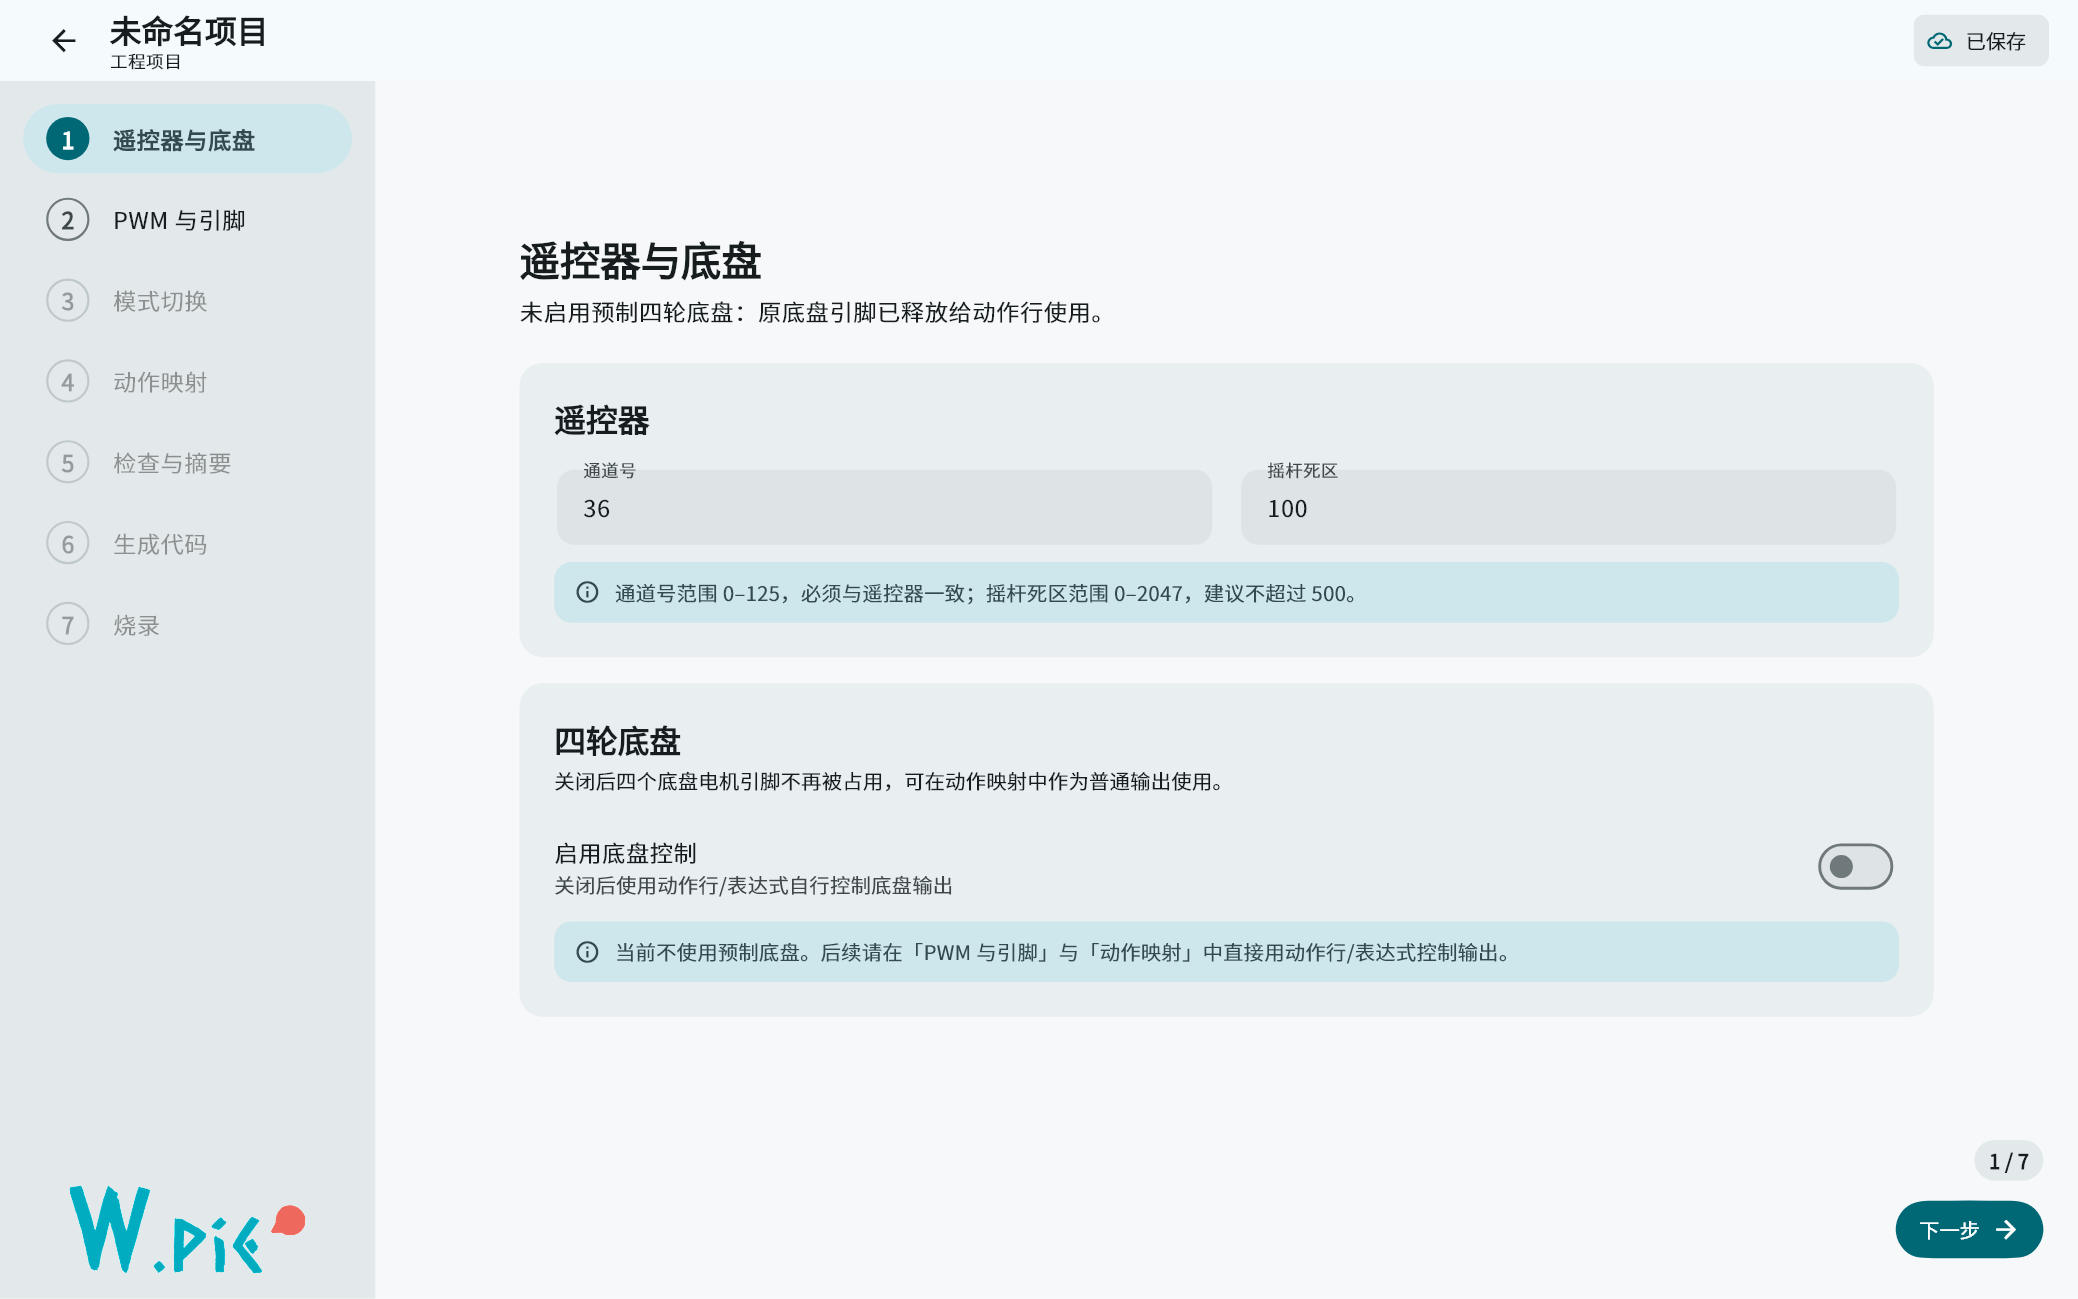
\includegraphics[width=0.95\linewidth]{image/ch05/5-1-chassis-off.png}
  \caption{工程项目关闭预制底盘后的“遥控器与底盘”页：原底盘引脚释放给动作行}
  \label{fig:concise-chassis-off}
\end{figure}

\section{引脚与频率}

“PWM 与引脚”页（图~\ref{fig:concise-pwm}）完成两件事：设置两组引脚的频率，指定每个
引脚的角色。

\begin{figure}[htbp]
  \centering
  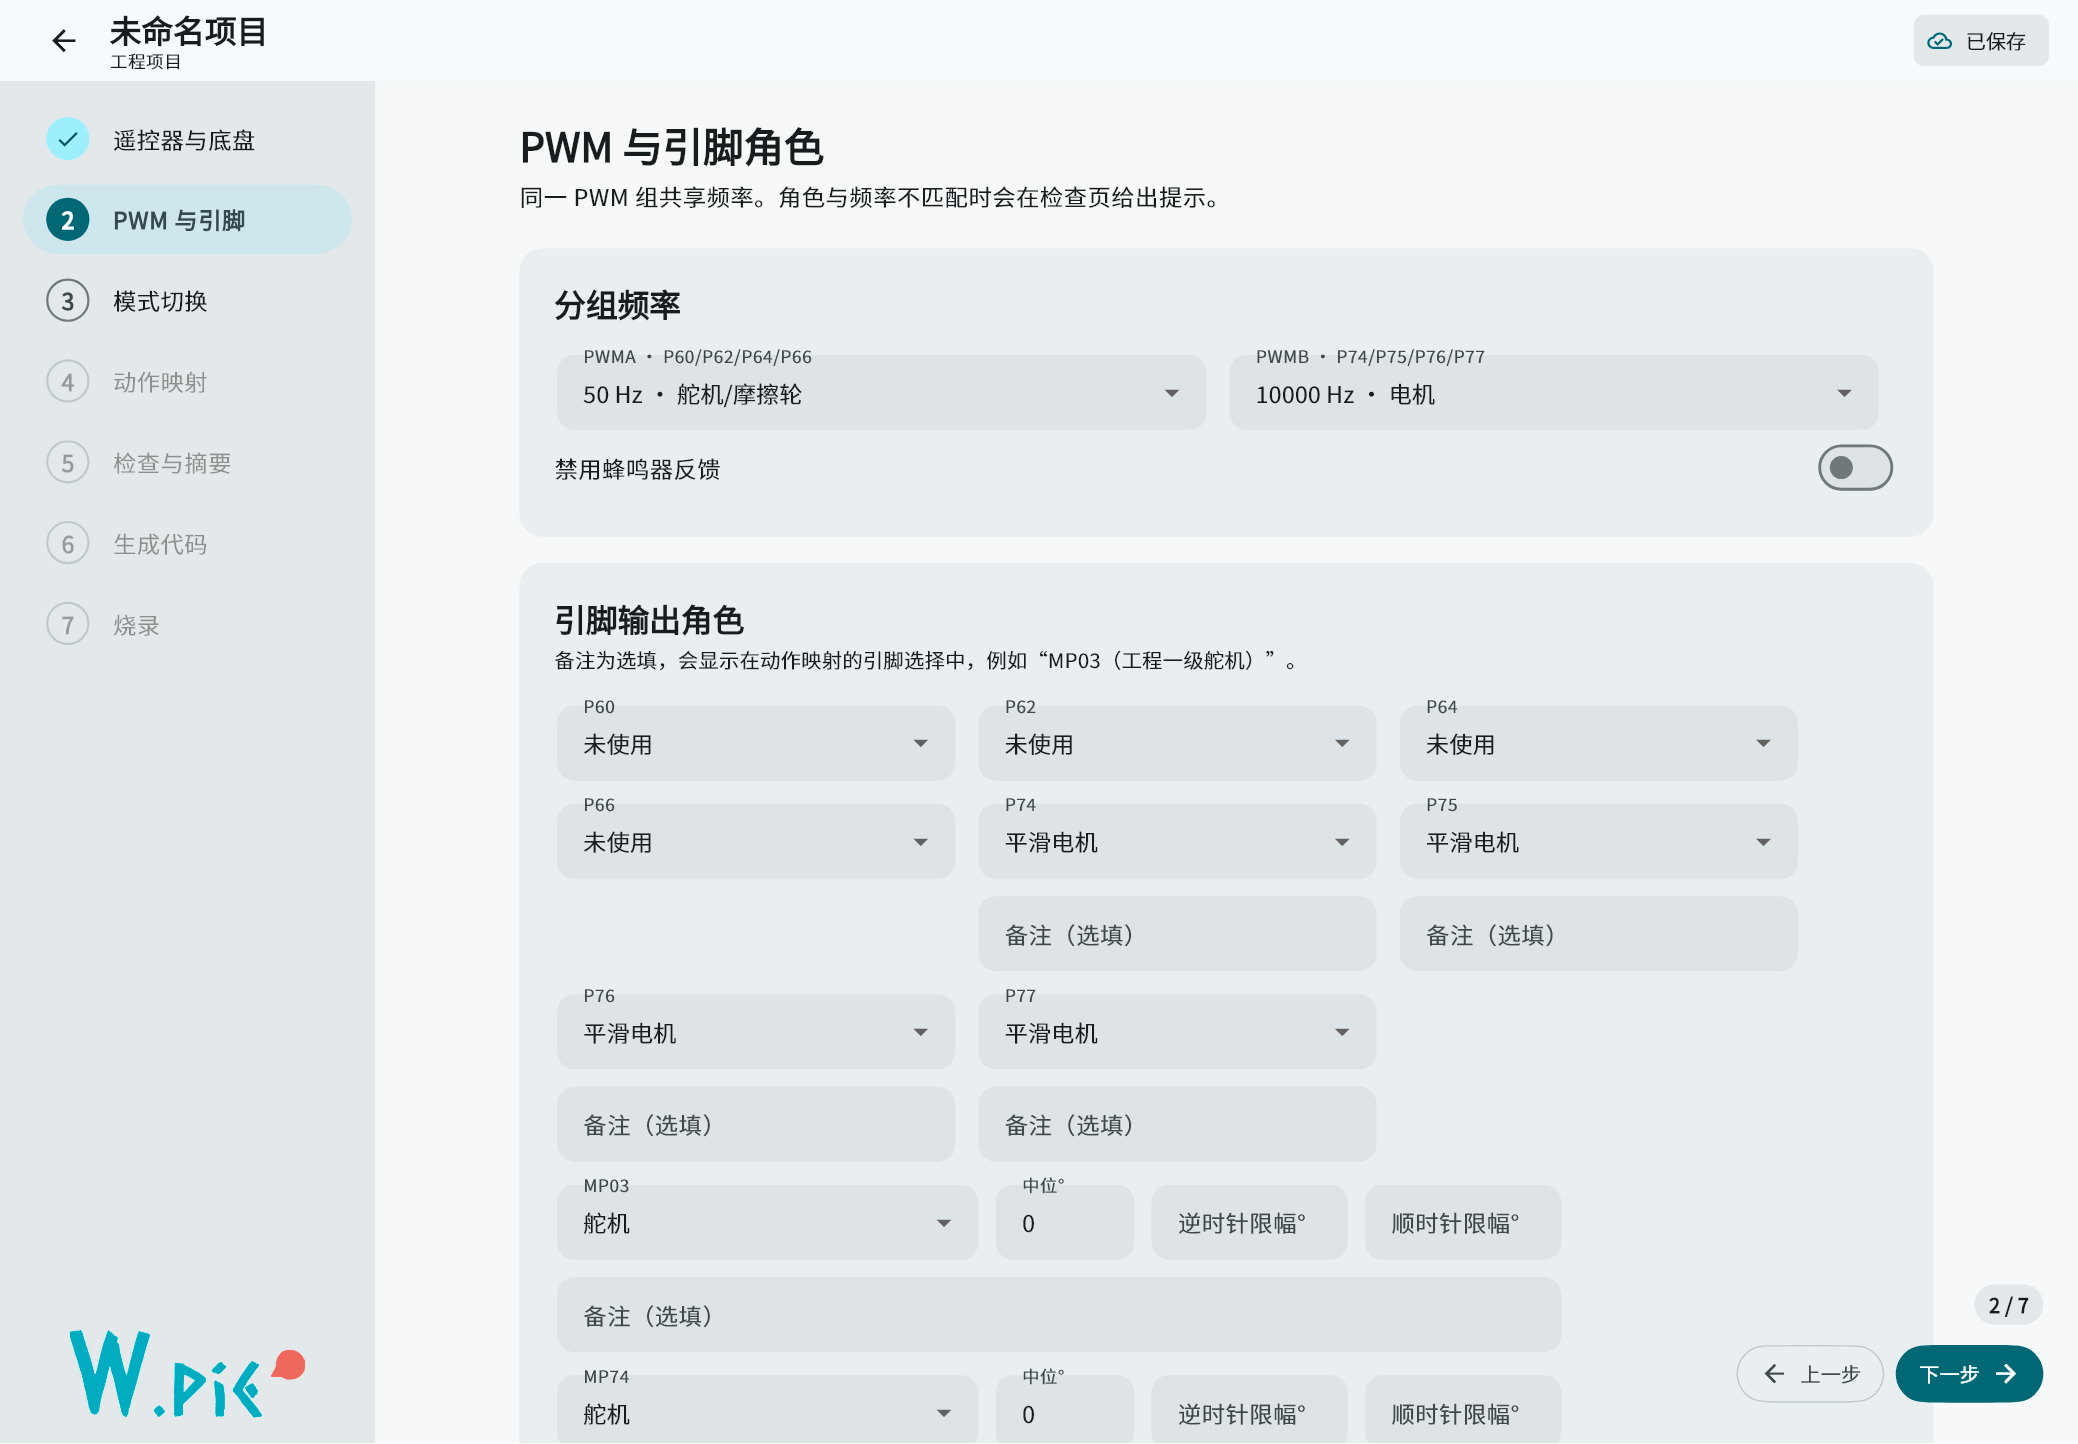
\includegraphics[width=0.95\linewidth]{image/ch05/5-2-pwm-pins.png}
  \caption{“PWM 与引脚”页：分组频率与每个引脚的输出角色}
  \label{fig:concise-pwm}
\end{figure}

同一组内的引脚共享频率：舵机与摩擦轮使用 50\,Hz 组，平滑驱动的电机使用 10000\,Hz 组。
角色与频率不匹配时，检查页会给出提示；不确定时保持默认分组即可。

每个引脚的可用角色由软件按硬件能力限定，下拉框只列出可用项。常用对应关系为：

\begin{itemize}
  \item P60、P62：电机、舵机或摩擦轮；
  \item P74--P77：电机、舵机或摩擦轮；
  \item P64、P66：舵机或摩擦轮；
  \item 主控板 MP03、MP74：舵机或摩擦轮。
\end{itemize}

引脚备注为选填项，只用于在动作行与动作表的下拉框中辨认用途，例如“工程一级舵机”；
备注不参与检查与动作执行。

\section{模式切换}

工程机器人可以设置 1--4 套互相独立的控制映射，用于不同任务。模式数量大于 1 时，需要
选择切换方式：

\begin{itemize}
  \item \textbf{单击轮换}：按同一个切换键，在各模式之间依次轮换；
  \item \textbf{一一对应}：为每个模式指定一个独立按键，按哪个键进入哪个模式。
\end{itemize}

每个模式的动作行与动作表相互独立。切换模式时，未被新模式映射的电机输出会清零，舵机
保持最后位置。因此每个模式都要把该模式需要的输出写全，不能依赖上一个模式的状态。

\section{动作行}

“动作映射”页按模式编辑动作。一个动作行由四部分组成：输入、输出、控制方式与参数。

\begin{itemize}
  \item \textbf{输入}：按键或摇杆轴；不指定输入时，该行只做变量计算；
  \item \textbf{输出}：动作作用的引脚，下拉框只列出已在“PWM 与引脚”页启用的引脚；
  \item \textbf{控制方式}：直接、单次、持续、速度、增速，或摩擦轮的启停、油门单次、
        油门持续、摇杆油门；下拉框只列出该引脚角色支持的方式；
  \item \textbf{参数}：按控制方式填写角度、速度、步长或油门百分比。
\end{itemize}

动作行按列表顺序执行，拖动左侧手柄可以调整顺序。建议一行只安排一个明确动作，先在
架空状态下逐行验证，再组合使用。动作行也支持用变量与表达式组合摇杆输入，用于自定义
混控；该写法不属于本简明版范围，需要时参见完整版教材。

\section{动作表}

动作表用于“一个按键走完一段流程”的机构，例如机械臂抓放、多档位伸缩。与动作行的
区别在于：动作表把一组输出按档位组织成表格，每按一次键前进一档，每个档位是一整列
完整的输出值。

\begin{itemize}
  \item 档位数可设为 2--8 档；
  \item “下一档键”负责前进，可选“上一档键”负责后退；
  \item “越界重复”开启时首尾循环，关闭时到首尾档停住；只有下一档键时固定循环；
  \item 表格按“引脚 × 档位”填写：舵机填带符号角度，电机填带符号速度，摩擦轮引脚
        填油门百分比；
  \item 卡片头部的复制键保留按键、档数与全部单元格，副本插入到源表之后；
  \item 档位较多、超出卡片宽度时，表格下方提供横向滚动条。
\end{itemize}

动作表是“写一次、保持”的控制方式：每档写入后保持，直到下一次按键切换。电机类关节
没有位置反馈，机械臂等机构必须配合机械限位与低速验证，不能只依赖档位数值。

\section{检查与实车验证}

工程项目的检查页会拦住引脚冲突、按键冲突、动作表缺格与越界等问题。由于控制逻辑由
使用者自行安排，检查通过只说明配置自洽，不说明动作符合机械结构，实车验证按以下顺序：

\begin{enumerate}
  \item 车体架空，可能干涉的机构拆下或脱离负载；
  \item 速度、角度、油门都取小值，逐行动作验证方向与幅度；
  \item 确认单个动作正常后，再验证同时输入与模式切换；
  \item 切换模式，确认未映射的电机停止、舵机保持，且没有意外动作；
  \item 全部通过后落地，先低速、空载运行，再逐步增加负载。
\end{enumerate}

\begin{note}
动作表与动作行都可能让机构持续出力。调试时保持手边可随时断电，出现异响、堵转或
超出行程立即切断电源，再回到配置中修改数值。机械限位是最后一道保护，不能省略。
\end{note}

\chapter{音乐项目}
\label{ch:concise-music}

\begin{introduction}
  \item 在钢琴卷帘中录入与编辑音符；
  \item 设置乐曲速度、拍号与重叠处理；
  \item 导入、导出 MIDI 并完成编译烧录。
\end{introduction}

音乐项目把主控板上的蜂鸣器变成一只可以演奏的喇叭。在钢琴卷帘中录入旋律，软件把它
整理成单音序列并生成固件；主控板上电后循环演奏，内置编译方式下还会在 OLED 屏上滚动
显示五线谱。它适合调试提示音、展示与教学，不参与机器人动作控制。

\section{钢琴卷帘}

音乐项目的第一步是钢琴卷帘编辑器（图~\ref{fig:concise-music}）。横轴是时间，纵轴是
音高，左侧一列钢琴键用于对照音高，画布上的色块就是音符。

\begin{figure}[htbp]
  \centering
  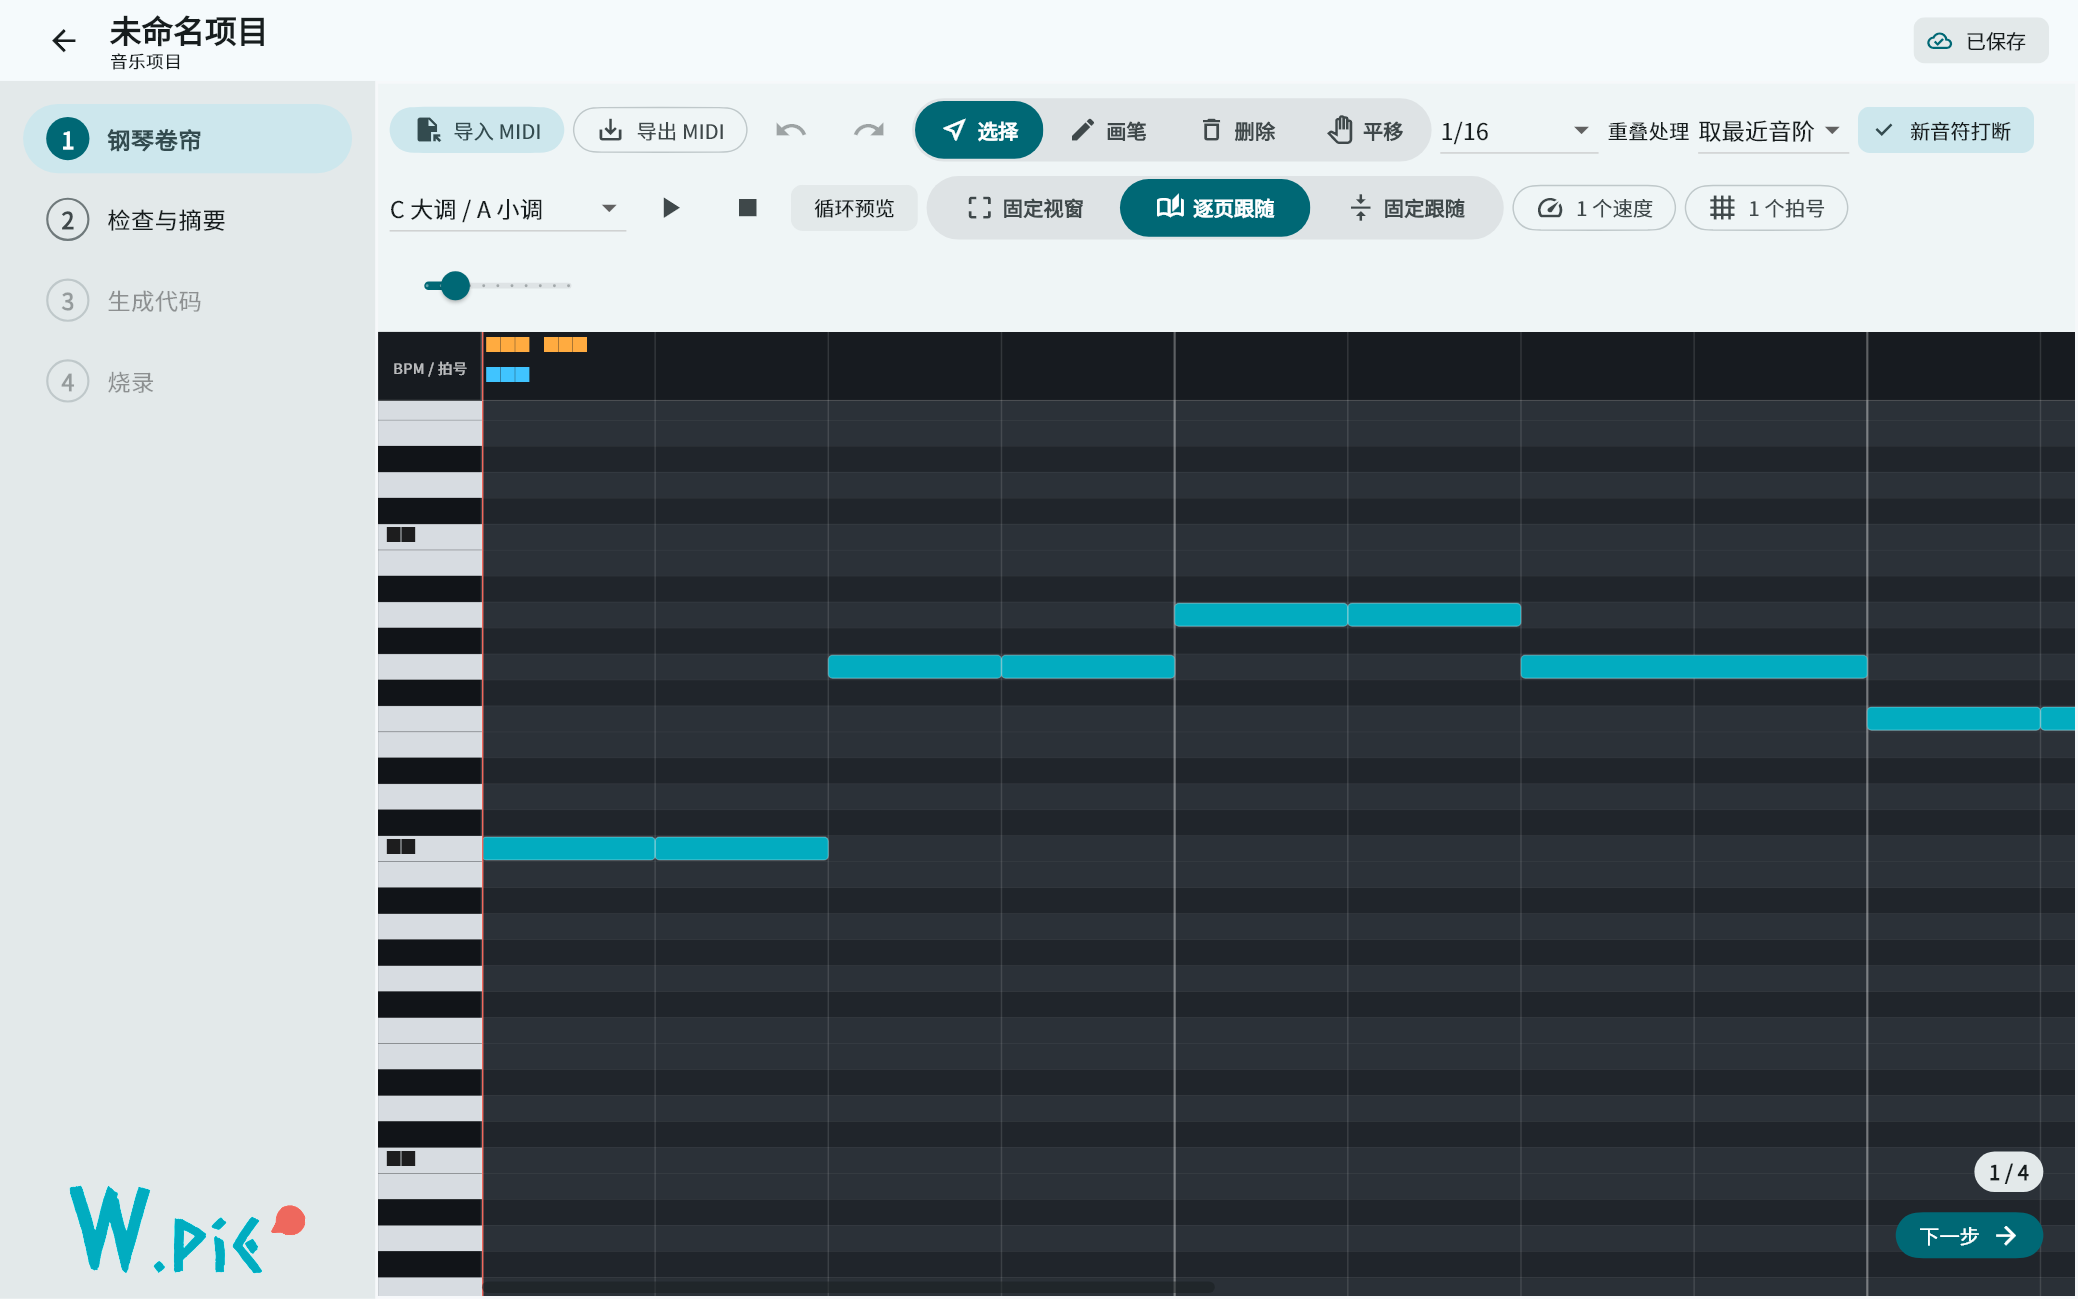
\includegraphics[width=0.98\linewidth]{image/ch07/7-1-music-editor.png}
  \caption{钢琴卷帘编辑器：工具栏、播放控制、速度与拍号事件以及音符区域}
  \label{fig:concise-music}
\end{figure}

工具栏提供四种编辑工具：\textbf{选择}用于点选与框选音符，\textbf{画笔}在网格上新建
音符并拖动改变时值，\textbf{删除}用于移除音符，\textbf{平移}用于整体移动选中的音符。
网格吸附决定新建与拖动对齐的刻度，可选十六分音符、三连音或不吸附。撤销与重做在编辑
过程中始终可用。

播放控制支持从任意位置试听；“循环预览”在编辑区内循环播放；“视窗跟随”让卷帘在播放
时自动跟随当前位置。预览与固件使用同一套发声规则，试听到的效果与主控板一致。

\section{速度与拍号}

工具栏第二行显示乐曲的速度与拍号事件。速度决定演奏的快慢，拍号影响五线谱的分小节
方式与显示。两类事件都从乐曲开头开始，按时间顺序排列；新增或修改后，检查页会核对
顺序是否合法。

初次使用时保持默认值即可，先录入旋律并试听，再根据需要调整速度。改变速度不会改变
音符的相对位置，只改变播放快慢。

\section{重叠处理}

蜂鸣器同一时刻只能发出一个音，而卷帘允许音符重叠。工具栏的“重叠处理”决定重叠时由
哪个音符发声：

\begin{itemize}
  \item \textbf{取最高音}：重叠时音高最高的音符发声；
  \item \textbf{取最低音}：重叠时音高最低的音符发声；
  \item \textbf{取最近音}：选择最接近上一个发声音高的音符，旋律连贯性较好。
\end{itemize}

打开“新音符打断”后，后开始的音符会打断仍在发声的音符，被打断的尾部不再发声。不发声
的音符在卷帘中显示为灰色；数据仍然保留，也参与导出，只是固件不播放。

\section{MIDI 导入与导出}

“导入 MIDI”从标准 MIDI 文件中选择一条旋律轨道，把音符、速度与拍号一并导入。文件里
如果有和弦，导入对话框会要求先选择重叠处理规则，再按规则保留一个声部。没有可用旋律
轨道时，导入会明确报错，不会生成空曲。

“导出 MIDI”把当前卷帘写成标准 MIDI 文件。重叠的完整数据也会写出，灰色音符在音频
软件中仍可编辑。音乐项目不保存原始 MIDI 的力度、乐器与通道信息，导出时值按最终发声
结果计算。

\section{生成与烧录}

音乐项目的“检查与摘要、生成代码、烧录”三步与其他项目一致。检查页会统计音符重叠并
提示采用的规则；曲目过长或音符过多时，会提示缩短乐曲。烧录完成后主控板上电即循环
演奏，内置编译方式下 OLED 屏同步滚动显示五线谱。

蜂鸣器音量有限，适合近距离试听与调试提示，不能替代功率放大后的扬声器。调整曲目后
重新编译烧录即可生效。


\appendix

% ------------------------------- 附录 ---------------------------------------
% 目录中附录编号前统一加“附录”前缀
\addtocontents{toc}{%
  \protect\renewcommand{\protect\cftchappresnum}{\appendixname\protect\space}%
  \protect\renewcommand{\protect\cftchapaftersnum}{}%
}

\chapter{检查、烧录与常见问题}
\label{app:concise-check}

\section{检查与摘要}

向导每一步都会实时检查当前配置，进入“检查与摘要”页时集中列出全部问题。问题分为两类：

\begin{itemize}
  \item \textbf{错误}：配置不完整或自相矛盾，阻止生成。常见原因包括通道号未填、同一
        引脚分配给两个设备、按键重复分配、必填项为空；
  \item \textbf{警告}：配置合法但可能不符合预期，只作提醒。常见原因包括冲刺速度偏低、
        拨弹电机位于低频引脚组、摩擦轮最大转速偏低、速度与引脚角色不完全匹配。
\end{itemize}

每条问题都带有定位信息，点击可直接跳回对应页面修改。修改后返回检查页，计数随之更新。
“配置概览”汇总通道、速度、引脚用途等关键配置，供生成前最后核对。

警告不等于错误，但也不应一律忽略。出现警告时，应确认当前方案确实接受该结果，再继续
生成；无法判断时，按警告提示调整配置。

\section{编译与烧录}

“烧录”页负责编译与写入。编译器一栏保持默认的内置编译器即可；已安装其他编译器的
使用者可以在下拉框中切换，但首次使用不建议改动。

页面提供三个操作：

\begin{itemize}
  \item \textbf{仅编译}：只完成编译，不写入主控板，用于确认配置与编译环境正常；
  \item \textbf{编译并烧录}：完成编译并写入已连接的主控板；
  \item \textbf{导出固件}：把编译结果保存为文件，供其他工具使用。
\end{itemize}

烧录前关闭主控板 SERVO、POWER 与机械拓展板 POWER、BOOSTER 四个供电开关，将主控板
断电后重新通过 USB 连接。页面检测到主控板后即可烧录；烧录成功后设备自动复位，检测到的
烧录设备消失属于正常现象。再次烧录前需要重新断电、上电。

Linux 首次烧录需要按页面提示安装设备访问权限；安装完成后重新插拔主控板。烧录失败时，
页面下方的进度与日志保留失败原因，可对照常见问题排查。

\begin{note}
只能烧录主控板。机械拓展板不运行用户固件，向拓展板烧录会破坏其出厂程序。烧录期间
不要插拔接线，也不要切换供电开关。
\end{note}

\section{装车前检查单}

以下检查单适用于步兵、工程与调试项目。每一项都能直接观察或操作，全部通过后才落地运行。

\begin{enumerate}
  \item 车体架空，轮子离地；弹仓清空，射界内无人；
  \item 关闭主控板 SERVO、POWER 与机械拓展板 POWER、BOOSTER 四个供电开关后连接 USB；
  \item 只向主控板烧录，确认烧录日志显示成功；
  \item 上电后听到启动提示音，确认程序已运行；
  \item 逐轮检查转向与整车方位一致，异常时修改配置而非现场改接线；
  \item 逐轴检查云台舵机方向与行程，确认不触碰机械限位；
  \item 检查拨弹电机方向与单发时长，确认卡弹时可反向退弹；
  \item 检查摩擦轮启动、加速与停止是否平滑，确认两侧转速无明显差异；
  \item 让测试序列或动作循环两轮，确认无偶发异常；
  \item 断电后再改接线或换设备；落地后先低速、空载运行，再逐步提速。
\end{enumerate}

\begin{note}
安全底线：不向机械拓展板烧录；不在上电状态插拔接线；摩擦轮最大转速不超过 800；
机构出现异响、堵转或超出行程时立即切断电源。机械限位是最后一道保护，任何时候都不能
省略。
\end{note}

\section{常见问题}

\begin{table}[H]
  \centering
  \small
  \begin{tabularx}{\linewidth}{@{}>{\raggedright\arraybackslash}p{0.28\linewidth}
      >{\raggedright\arraybackslash}X@{}}
    \toprule
    现象 & 处理 \\
    \midrule
    车完全不动 & 确认手柄与主控板均已上电；核对通道号是否一致；检查死区是否过大；确认
      烧录成功 \\
    前进却后退 & 摇杆极性可能与配置相反；架空低速核对，必要时调整方向或转向设置 \\
    个别轮子反向 & 修改该轮的“方向”，不改接线；四个轮子同时反向时先核对整机前后约定 \\
    转向相反 & 打开“反转左右转向”，前后移动不受影响 \\
    拨弹一卡一卡 & 拨弹电机位于低频引脚组，属正常现象；提高拨弹速度、缩短单发时长，
      或改用连续拨弹 \\
    摩擦轮带不动 & 检查最大转速是否偏低、机械阻力是否过大；电调首次使用需完成油门
      行程学习 \\
    未检测到主控板 & 关闭四个供电开关；主控板断电后重新上电；更换 USB 口与数据线，
      避免经过集线器 \\
    烧录中断或写块无响应 & 更换 USB 口与数据线；关闭占用设备的其他程序；重新断电
      上电后重试 \\
    首次编译失败 & 检查项目路径与缓存目录是否包含中文字符；把工具目录加入杀毒软件
      白名单后重试 \\
    Web 版不能烧录 & 浏览器无法访问本地设备；配置与检查可在 Web 版完成，编译烧录
      回到桌面版 \\
    模式切换后轮子停 & 新模式没有映射这四路输出；在动作映射中补全该模式需要的输出 \\
    旧项目打不开 & 旧版本存档可能不被当前版本接受；用对应旧版打开并另存，或按新版本
      重建配置 \\
    \bottomrule
  \end{tabularx}
  \caption{常见问题速查}
  \label{tab:concise-faq}
\end{table}


\end{document}
